%************************************************
\chapter{Information Theory}\label{ch:information}

%************************************************
\begin{quotation}
	\small \emph{ \flushright Only through communication can human life hold meaning.\\
	\flushright --- Paulo Freire\\
	\vspace{1cm} }
\end{quotation}
This chapter derives Shannon Information from Probability Theory, explicates some implicit assumptions in the usage of Shannon Information, and explains basic Information Theory concepts.


\section{From Probability to Information}\label{sec:prob2info}
In \cref{sec:anatomy_ia}, we exposed that an agent updates its model of the world from sensory data, experience. We have also shown how this update happens; a sceptical agent \emph{proportions her beliefs to the evidence} according to Bayes' theorem.

The amount of this update on knowledge is not uniform. Some experiences are more valuable than others, i.e.\ some evidence will produce a bigger change in the agent's knowledge, leading to a greater impact in her future actions. We say that those experiences are more informative.
\begin{definition}\label{def:information}
	\textbf{Information} is what changes belief~\cite{sowinski:2016,caticha:2008}.
\end{definition}

Let us say that an agent's \emph{prior} belief in a statement \(S\) is \(P(S) \)\footnote{\(P(S) \) is in fact \(P(S|K) \), but we supress it to reduce the clutter.}. After experiencing some evidence \(\re\), her \emph{posterior} set of beliefs is updated to incorporate the evidence, \(P(S|\re )\)\footnote{Here we are talking about \emph{events}: \(P(S|\re )\) is a short hand for \(P(S|\{\re\} \land K )\).}. The prior and the posterior are related by the product rule (\cref{sec:independent_events})~\cite{sowinski:2016}:
\begin{align}
	\underbrace{P(S|\re)}_{Posterior}&= \frac{P(\re | S )}{P(\re)}\cdot \underbrace{P(S)}_{Prior}
\end{align}

We shall call this ratio by which prior and posterior are related as likelihood (\(\LH\)):

% % This update procedure can be generalised to a set of experiences. Consider a sequence of experiences: \(E = \{\re_t\}_0^T\)
% % \[p(S|\re_0) \to p(S|\re_0 \land \re_1) \to \cdots \to p(S|\re_0 \land \re_1 \land \cdots \land \re_T)
% %   \]
% % But according to the Cox axiom~\ref{consistency}~\ref{axiom:order}, an agent may partition her experiences in any way she chooses, and this does not affect her final belief~\cite{sowinski:2016}. Therefore\footnote{We have already ( section~\ref {sec:skeptical_agents}) delved a little on the implications of the indifference to the order of evidence which is also an indifference in sequential versus simultaneous updating.}:
\begin{align}
	\LH(\re; S) &= \frac{\text{Posterior}}{\text{Prior}} = \frac{P(S | \re )}{P(S)} = \frac{P(\re | S )}{P(\re)} \label{eq:likelihood}\\
	P(S|\re ) &= \LH(\re; S)\cdot P(S).
 \end{align}
Simply by observing equation~\ref{eq:likelihood}, we can conclude that if information (\(i\)) is what changes belief, information and likelihood must be related to one another:
\begin{align}
	i_S(\re) = f(\LH(\re; S)).
\label{eq:information_as_function_of_likelihood} \end{align}

Moreover, if an experience does not change a belief, it contains no information: \(f(1)=0\).

We also hope that when the likelihood changes by an infinitesimal amount, the information does not change discontinuously, so \(f\) is continuous.

The information gathered from independent \emph{events} must reflect the commutativity of Cox's axiom~\ref{consistency}~\ref{axiom:order}. Let \(\LH_1 = \LH (e_1; S)\) and \(\LH_2 = \LH (e_2; S)\), information must satisfy the functional constraints~\cite{sowinski:2016}:
\[
\begin{cases}
	f(\LH_1 \land \LH_2) &= f(\LH_1) + f(\LH_2)\\
	f(1) &= 0\\
	f &\text{is continuous.}
\end{cases}
\]
This functional form can be solved and its solution is~\cite{caticha:2008}:
\begin{align}
	f = A \cdot \ln{\LH(\re; S)} \therefore \nonumber\\
	i_S(\re) = A \cdot \ln{\LH(\re; S)}.\label{eq:i_equals_log_LH}
\end{align}
From equations~\ref{eq:i_equals_log_LH} and~\ref{eq:likelihood},
\begin{align}
	i_S(\re) &= A \cdot \ln{ \frac{P(S | \re )}{p(S)}}\\
	i_S(\re) &= A \cdot \ln{ P(S|e )} - A \cdot \ln{p(S)}.
\label{eq:is_ln} \end{align}
The constant \(A\) allow us to use any base \(b\) in the logarithm:
\begin{align}
	A = \frac {1}{\ln b} \to i_S(\re) = \log_b P(S|\re ).
\end{align}
We can argue that the ammount of information gained by the agent about the world is equivalent to some ammount of \emph{hidden information} \(h\) that was revealed to the agent by the \emph{event} \(e\).

Hence, \(i_S(e)=-\Delta h(e)\), from eq.~\ref{eq:is_ln}:
\begin{align}
	i_S(e) &= \log{ P(S|e )} - \log {P(S)} \\
	i_S(e) &= - \left[ \biggl(\underbrace{-\log{P(S|e )}}_{h(S|e )}\biggr) - \biggl(\underbrace{-\log{P(S)}}_{h(S)}\biggr) \right] \\
	i_S(e)&=-\Delta h(e).
\end{align}

Delightfully, our definition of \emph{hidden information} that reduces the uncertatinty of the agent, and emerged from our definition of information,
\begin{align}
	h (S) = - \log P(S)
\end{align}
is equivalent to Shannon's self information\footnote{Also known as the Shannon information content of an outcome~\cite{mackay:2002}.}:
\begin{align}
	I[\src] = - \log p(\rs)
\end{align}

In \acf{IT}, self-information is defined as the entropy contribution of an individual message (or symbol); in other words, how much uncertainty reduction can be attained by an individual \emph{event}. This uncertainty reduction is precisely what we derived.

\textbf{Shannon's information can be derived from probability theory.}\label{sec:probability2information}$\qedhere$

\section{Expliciting the implicit assumptions} When we derived Probability Theory from a language for rational agents, and then Information Theory from Probability Theory, we exposed their assumptions. Including \textbf{consistency}:
\begin{enumerate}
	[i.]
	\item A belief in a statement can not depend on the path used to arrive at it. In other words, it does not matter the order in which evidence is presented.
	\item No evidence can be arbitrarily ignored.
	\item Statements which are known to be identical must be assigned the same degree of belief.
\end{enumerate}

When we use these theories to ground Machine Learning Theory, we are \textbf{implicitly accepting} the assumptions above. Symbolic AI guarantees that their agents follow such assumptions by construction.

We know humans do not follow these assumptions, and the whole point of conceptualising rational agents was to study a simplified form of intelligence. For humans,
\begin{enumerate}
	[i.]
	\item the order in which we experience pieces of evidence matter~\cite{wiesel:1982};
	\item we forget or suppress past experiences;
	\item we can change our mind even in the absence of new evidence.
\end{enumerate}
What about \aclp{DNN}?

There is nothing by construction that forces \acsp{DNN} to be consistent. Recent findings~\cite{achille:2018critical} show that, in \acsp{DNN}, the order in which evidence is presented has a significant effect on the learning result. Therefore, we conjecture:
\begin{conjecture}
	A complete learning theory of \acf{DL} has to address \textbf{time} and its effect on the \textbf{cost} of changing a belief.
\end{conjecture}


\section{Shannon's Mathematical Theory of Communication}

% \subsection{A \emph{bit} of fiction}
\acf{IT} has an identifiable beginning: Shannon's 1948 paper~\citeauthoritle*{shannon:1948} was a giant leap towards understanding communication and defining \emph{information}\footnote{In a rare piece of collaboration, Shannon asked his lunchroom table colleagues at Bell Labs to come up with a snapier name than \emph{binary digit}. \emph{Bigit} was considered, but John Tukey's proposal, \emph{bit}, was chosen~\cite{soni:2017}.}. Despite his acknowledging of the influence from previous works by pioneers such Harry Nyquist and Ralph Hartley, it was Shannon's unifying vision that revolutionized communication and provided a \emph{``blueprint'} for the information age~\cite{aftab:2001}. His theory defines unbreachable limits, the \emph{``laws of information''}~\cite{stone:2015}:

	\begin{enumerate}[i.]\label{shannon_laws}
		\item There is an upper limit, the \textbf{channel capacity}, to the amount of information that can be communicated through the channel;
		\item \textbf{Noise} reduces the \textbf{channel capacity};
		\item There is an encoding that allows \textbf{lossless} communication trough a \textbf{noisy channel}.
	\end{enumerate}

The idea that it is possible to transmit information with zero error through a noisy channel is not at all intuitive, and its theoretical proof was an unexpected result at the time. In the following sections, we will explain the concepts of \ac{IT} that allow us to comprehend these \emph{laws of information}.

\subsection{The communication problem setting}\label{sec:communication_problem_setting}

Shannon deliberately chose not to deal with fuzzy concepts as intelligence or meaning:
\begin{quotation}
	\small \emph{ \textbf{The fundamental problem of communication is that of reproducing at one point either exactly or approximately a message selected at another point.} Frequently, the messages have meaning; that is, they refer to or are correlated according to some system with certain physical or conceptual entities. These \textbf{semantic aspects of communication are irrelevant to the engineering problem}. The significant aspect is that the actual message is one \textbf{selected from a set} of possible messages.\\
	\flushright --- Claude Shannon,~\citeauthoritle*[p.1]{shannon:1948}\index{Claude Shannon}\\}
	\vspace{1cm}
\end{quotation}

Conceptually, this setting can be explained as follows (\cref{fig:communication_setting}): \footnote{\(\srcsymb\) is the intended message. One can think about it as the meaning or the semantics.}

\begin{figure}[hbt!]
	\centering
	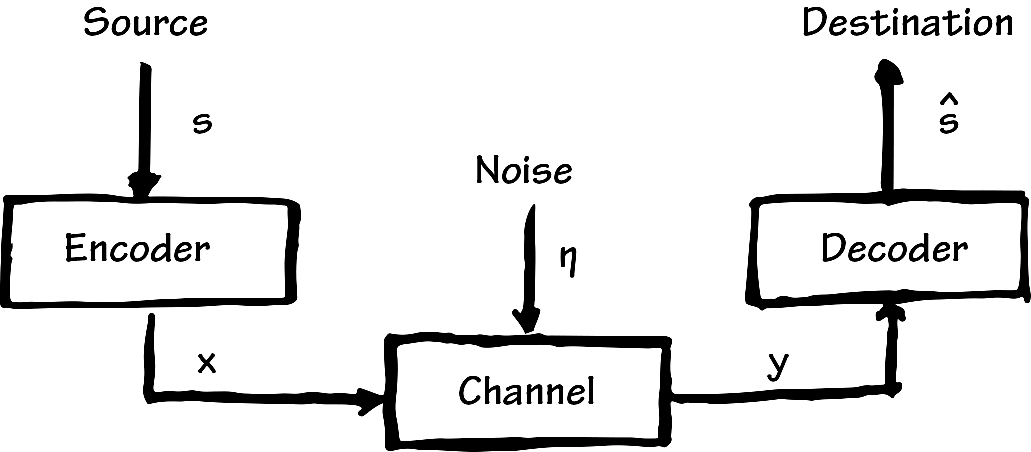
\includegraphics[width=\textwidth]{communication_setting}
	\caption{The communication problem setting.}\label{fig:communication_setting}
\end{figure}


The Source:
\begin{enumerate}
	\item selects a message  $\srcsymb$ from a set of possible messages $\srcalph$,
	\item encodes the message $\srcsymb$ into a string of symbols $\encsymb$, the signal,
	\item transmits this string of inputs $\encsymb$ through a noisy channel.
\end{enumerate}
\footnote{\(\srcalph\) is the alphabet or the set of possible outcomes of the random variable \(\src\).}

The Destination, then:
\begin{enumerate}
	\item receives a string of symbols \(\decsymb\),
	\item decodes the string \(\decsymb\) into the most probable message \(\hat{\srcsymb}\).
\end{enumerate}

\section{Information} The reason for communication is to change another agent's behaviour. In other words, \emph{communication either affects the conduct of the recipient, or it is like it has never happened}~\cite[p.100]{shannon:1948}. We have already established (\cref{sec:prob2info}, definition~\ref{def:information}) that \emph{information is what changes belief}; thus, changes an agent's conduct. So, \textbf{communication is transmitting information}.

Noteworthy, information is independent of the \emph{enconding} or the channel chosen. One can use any language (English, Portuguese, music, images, dance, etc.) and any means of transmission (letter, telegraphy, microwaves, etc.) that the transmitted information remains the same.

To simplify, Shannon constrained semantics to the act of choosing a message from a set of finite possibilities. A source (a person, a machine or phenomenon) that always sends the same message never surprises the receiver, and the message carries no information. On the contrary, a source that sends symbols at random is impossible to predict and, therefore, every message carries maximal information.

Therefore, in this setting, \emph{information is a measure of freedom of choice in selecting the message}~\cite[p.100]{shannon:1949}. In other words, it is a measure of surprisal or uncertainty reduction.

In the aforementioned famous paper, Shannon limited to say that mathematically, if the set of possible messages \(\srcalph\)  is finite, any function of the size of this set \(f(|\srcalph|)\) is a measure of information and that the logarithmic function is a natural choice. We shall expand on this idea.

\subsection{A guessing game}\label{guessing_game} Imagine a number from 1 to 1000. Let us assume that you picked the number at random. Thus, each number in the range had the same chance of being chosen, \(\frac{1}{1000}\). How many questions do I need to ask to guess your number correctly? Well, it depends on what are the allowed answers. I could ask:
\begin{wrapfigure}
	{L}{0.5
	\textwidth} \centering
	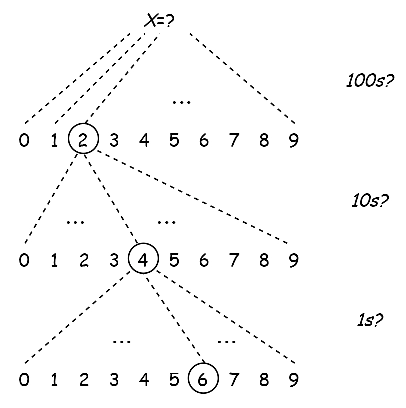
\includegraphics[width=0.45
	\textwidth]{246}
	\caption{Branching factor of 10 to find 246.}\label{fig:branching} \end{wrapfigure}
\begin{itemize}
	\item How many hundreds do your number have?
	\item Then, I would ask how many tens do your number have?
	\item Then, how many units?
\end{itemize}

In this case, the number of questions needed is three, the height of the tree in \cref{fig:branching}, because we allowed each answer to be a \emph{digit}; therefore, the \emph{branching factor} \(b\) of the decision tree was 10. It is easy to notice that the tree's height is \(\log_b (1000)\).

It is now clear what Shannon meant by saying that the logarithmic function was the natural measure of information. The logarithm will give the height (number of questions) of the decision tree based on the number of possible answers (the logarithm base). The branching factor is just a measurement unit and can be chosen arbitrarily.

The smallest branching factor is 2, a \emph{bit}. So, one bit is the amount of information that resulted from choosing between two equally likely options.

To solve the same guessing game with \emph{bits}, \ie with yes or no questions, one proceeds with a binary search, and in the worse case it will need \(\log_{2}(1000)=\frac{\log_{10}(1000)}{\log_{10}(2)}\approx 9.96 \therefore 10\) questions.

How about if the choice was among not equally likely options? Let us examine the simplest case of an unfair coin.

\Tree [.\(\rvX\)? [\(P(\rvX=H)=75\%\) \(P(\rvX=T)=25\%\) ] ]\\

Here, we expect the outcome to be \emph{heads}, so if it turns \emph{tails}, we get surprised. Before the coin flip, we were 25\% certain (our belief measure) that the \emph{experiment} would turn \emph{tails}. If it, in fact, turns \emph{tails}, our certainty reaches 100\%, growing by a factor of \(\frac{1}{0.25}=4\). So it is reasonable to think that our uncertainty of the \emph{tails} outcome decreased by a factor of 4 as well. We were 75\% certain that the \emph{experiment} would turn \emph{heads}. If it in fact turns \emph{heads}, our uncertainty of the \emph{heads} outcome decreased by a factor of \(\frac{1}{0.75}\approx 1.\overline{3}\). How do we transform this uncertainty reduction factor to a measure in bits? In other words, how do we measure in bits the information gained by unveiling an outcome?

Notice that 1 \emph{bit} is the amount of information that reduces uncertainty from 2 possible states to 1, a factor of 2. Also, 2 bits of information reduce the uncertainty from the 4 possible representable states with 2 bits to 1, a factor of 4.
\begin{align*}
	2^1 \text{ factor} &=  1\text{ bit} \\
	2^2 \text{ factor} &=  2\text{ bits} \\
	\cdots\\
	2^n \text{ factor} &= n\text{ bits}  \\
	\therefore x \text{ factor} &= \log_2 (x) \text{ bits}
\end{align*}
So, if an outcome has probability \(p(\encsymb)\):
\begin{align*}
	\frac{1}{p(\encsymb)} \text{ factor}  \implies \log_2 \frac{1}{p(\encsymb)} \text{bits} = - \log_2 p(\encsymb) \text{ bits}
\end{align*}

If the factor is a measure of the reduction in freedom of choice, the factor is the information gained by knowing the outcome of the \emph{experiment}. This factor is known as \textbf{self-information} or information content of an outcome\footnote{Information theory magnitudes are functions of the probabilities random variables and not directly of a random variable. To address this difference, we opt to use square brackets instead of parenthesis.}:
\begin{definition}\label{def:surprisal}
	The \textbf{information content, self-information, surprisal}, or \textbf{Shannon information} of a particular outcome \(\encsymb\) of an \emph{experiment} is defined as:
	\begin{align}
		I[\encsymb] = h[\encsymb]= -\log p(\encsymb)\\
		\tag{information content of outcome}
	\end{align}
\end{definition}
As we already had derived in \cref{sec:probability2information}.

\subsection{Entropy} In practice, however, we are not usually interested in the information of a particular outcome, but in how surprised, on average, we will expect to be with the entire set of possible outcomes.
\begin{definition}
	The entropy \(H[\rvX]\) of a random variable \(\enc\) is defined to be the average Shannon information content of its possible outcomes:
	\begin{align}
		H[\rvX] \eqdef \E_p \frac{1}{\log p(\encsymb)} = -\sum_{\encsymb \in \encalph} p(\encsymb) \log p(\encsymb) \text{ bits/symbol}.
	\label{eq:entropy} \end{align}
\end{definition}
\footnote{We will constrain our explanations of Information Theory to the discrete case. It can be argued that if we are interested in models that computers will use, some quantisation will always happen.}
Entropy can be seen in two ways:
\begin{enumerate}
	\item as the quantity of information ``produced'' by the source~\cite[p.18]{shannon:1949}.
	\item as a measure of \emph{uncertainty} or lack of pattern.
\end{enumerate}
Average information shares de same definition as Entropy; therefore, to know whether a quantity is information or Entropy depends on whether it is given or taken~\cite{stone:2015}. In other words, uncertainty reduced is information gained, and vice-versa. If a random variable \(\enc\) is very uncertain, then it has high Entropy. If we are told the outcome of the variable \(\rvX = \encsymb_j\), we have been given information that is equal to the uncertainty we had. Thus, receiving an amount of information is equivalent to having the same amount of Entropy taken away.

\section{The source} In the problem setting proposed by Shannon, the source generates a message, symbol by symbol. The choice of each symbol depends on the ``preceding choices as well as the particular symbols in question''~\cite[p.10]{shannon:1949}.

A mathematical model that follows this description is known as a \emph{stochastic process}. Any discrete source can be represented by a stochastic process. ``Conversely, any stochastic process may be considered a discrete source''~\cite{shannon:1949}.
\begin{definition}
	A \textbf{stochastic (or random) process} is a set of random variables indexed by a variable \(i \in \Natural\) (usually representing time):
	\begin{align}
		{\src_i}, i \in \Natural \\
		\tag{Stochastic Process}
	\end{align}
\end{definition}

In the original formulation, Shannon modeled the source as a stochastic process indexed by time. He thought the source as an entity that emits a certain rate, amount of information (bits) per period (seconds):
\begin{align}
\srcrate \eqdef \frac{H[\src]}{T_{\src}} \frac{\text{ bits}}{\text{ second}}
\end{align}
where \(T_{\src}\) is the average time in seconds of transmitting a symbol.
For simplification sake, from now on we will just say that the source rate is:
\begin{align}
	\srcrate = H[\src] \text{ bits/symbol}
	\end{align}
% We describe a stochastic process as \(\rvX_t = [\sA_{\rvX_t}, p_{\rvX_t}]\), where \(\sA_{\rvX_t}=\{\encsymb_t\}, t \in \sT\) is the alphabet from which the process chooses the symbols to emit; and \(p_{\rvX_t}=\{p_t\}, t \in \sT \) are the probabilities of choosing each symbol.

\subsection{Markov chains} More specifically, Shannon proposed using a special kind of stochastic process called an \emph{ergodic Markov chain} to model the source.
\begin{definition}
	An order-k \textbf{Markov chain} is a stochastic process that satisfies the following property:
	\begin{align}
		P(\src_i|\src_{i-1}, \src_{i-2}, \cdots, \src_{i-k})=P(\src_i|\src_{i-1}, \src_{i-2}, \cdots, \src_1)
	\end{align}
	The \textbf{ergodic} property means statistical homogeneity~\cite{shannon:1949}: its statistical properties can be deduced from a single, sufficiently long, random sample of the process.

\end{definition}
An order-k ergodic Markov chain is a process with a memory of \(k\) states. By modelling the source as an ergodic Markov chain, Shannon showed that his theory not only works for phenomena that can be modelled as i.i.d. random variables. The source can behave like a chain of random variables \( \{\src\}\), each representing an outcome \(\srcsymb \in \srcalph\) that are dependent on each other, as long as the sequence produced is longer than the number of symbols needed to the Markovian process achieve its stability.


\section{The encoder: Data compression}
\begin{quotation}
	\small \emph{ \flushright What’s in a name? \\
That which we call a rose,\\
by any other word would smell as sweet.\\
	\flushright --- Romeo and Juliet (act.2, sce.2), William Shakespeare\\
	\vspace{1cm} }
\end{quotation}
An encoding transforms information into data. The same information can be transformed into an audio file with spoken English, a piece of writing in Portuguese, or even an image. These encodings represent the information uniquely and differ in the amount of data (\emph{bits}) they use.

	\begin{figure}[hbt!]
		\centering
		\makebox[\largefigure][r]{
		\centering
		\begin{subfigure}
			[b]{.27\largefigure} \centering
			
\includegraphics[width=
			\textwidth]{cutia-photo}
			\caption{360 Kb 15\small{cm}x20\small{cm} PNG colored image of a cat.}
		\end{subfigure}
		\hspace*{1em}
		\begin{subfigure}
			[b]{.27\largefigure} \centering
			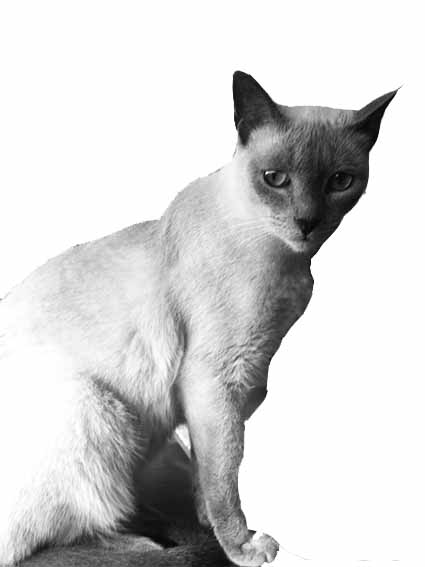
\includegraphics[width=
			\textwidth]{cutia-gray}
			\caption{  27 Kb 15\small{cm}x20\small{cm} JPG grayscale image of a cat.}
	\end{subfigure}
		\hspace*{1em}
		\begin{subfigure}
			[b]{.2733\largefigure} \centering
			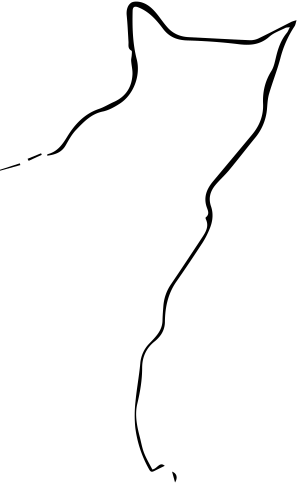
\includegraphics[width=
			\textwidth]{cutia-line}
			\caption{4.9 Kb 15\small{cm}x20\small{cm} SVG duotone image of a cat.}
	\end{subfigure}
	\hspace*{3.3cm}
}
\caption{Different representations of a cat and their encoding sizes in bits.}
\end{figure}




This idea may be better explained with an analogy with natural languages. Languages encode ideas into words in different ways~\cite{zaslavsky:2018}. For example, while in English's \emph{``to be''} is universal, Portuguese has two different verbs: \emph{``ser''} and \emph{``estar''}; the first for permanent, unchanging cases; the second for temporary situations such as mood or weather. At the same time, similar or identical
Meanings appear in unrelated languages~\cite{zaslavsky:2018}.

Thus, a message in a natural language can be translated (encoded) to another language and both messages will hardly have the same number of words, characteres, or size in \emph{bits}:
\begin{align}
	\srcblk=\{\src_1, \cdots, \src_n\}&~\underrightarrow{~encoding~}~
	\{\enc_1,  \cdots, \enc_k\}=\encblk.\\
\end{align}

Besides, some symbols are more important in a message: ``Mst nglsh spkrs wll ndrstnd ths phrs wtht vwls\footnote{``Most English speakers will understand this phrase without vowels''.}''. Here we created \emph{codewords} for words in English that a receiver can understand by the context (and certainly if she has a \emph{codebook}\footnote{A \emph{codebook} is a dictionary that relates words in the source alphabet, \(\srcalph\) to words, codes, in the encoder alphabet\(\encalph\).}).

Shannon's source coding theorem is about encoding messages efficiently, a form of data compression~\cite{stone:2015}. Here we present some definitions that will help us understand the theorem later.

\begin{definition}
A \textbf{(m, k) block code}, also known as a codebook, is a set of \(m\) codewords represented by a sequence of \(k\) bits:
\begin{align}
\{\enc^k(1),\enc^k(2),...,\enc^k(m)\},~\enc^k(i) \in \encalph^k, ~m \in \Natural.
\end{align}
\end{definition}
\begin{definition} The rate \(\sR_{\text{code}}\) of a (m,k) code is:
	\begin{align}
		\sR_{\text{code}} = \frac{\log m}{k}~\frac{\text{bits}}{\text{symbol}}\label{code_rate}
		\end{align}
\end{definition}
\begin{definition}
Let \(\srcblk\) be a block of \(n\) random variables, representing consecutive symbols \(\src_i \in \srcalph\) emited by the source. A \textbf{binary block encoder}  \(\enc\) is a function:
\begin{align}
	\enc:~ \srcalph^n \to {\{0,1\}}^k
\end{align}
that ``translates'' the block of source symbols (the message) into a code \(\encblk\) of \(k\) bits, using a \((|\srcalph^n|, k)\) code:
\begin{align}
	\enc(\srcblk)=\{\encsymb_1,  \cdots, \encsymb_k\}=\encvec \in {\{0,1\}}^k
\end{align}
\end{definition}
\begin{definition} The rate \(\encrate\) of a binary block encoder is:
	\begin{align}
		\encrate = \frac{\log |\srcalph^n|}{k}=\frac{n}{k}\log |\srcalph|~\frac{\text{bits}}{\text{symbol}}
		\end{align}
\end{definition}

% The efficiency of an encoder is its rate, how many useful bits it transforms per souce period (\(T_{\src}\)):
% \begin{align}
% 	n \text{symbols} = k \text{bits}\\
% 	\frac{n}{T_{\src}} \frac{\text{symbols}}{\text{seconds}}= \frac{k}{T_{\src}} \frac{\text{symbols}}{\text{seconds}}
% \end{align}

% The efficiency of the encoding \(\rvX^{k}\) can be defined by the rate:
% \begin{align}
% 	R_{\rvX} = \frac{k}{n} \frac{\text{bits}}{\text{symbol}}
% \end{align}
% Shannon's source coding theorem is essentially about data compression~\cite{stone:2015}.
% The encoding process yields inputs with a specific distribution \(p(\rvX)\). The shape of this distribution determines its entropy \(H[\rvX]\) and therefore how much information each input carries\cite{stone:2015}.

% We can interpret Shannon's source coding theorem in terms of data compression.  This interpretation was developed independently by Russian mathematician Andrey Kolmogorov(1933). He defined algorithmic complexity to be the length of the shortest computer program capable of describing a given object (e.g a message).  Algorithmic complexity is now known as Kolmogorov complexity\cite{stone:2015}.

% The encoding process yields a specific distribution \(p(\encsymb)\) to the channel input \enc. The distribution determines its entropy \(H[\rvX]\) and therefore how much information each symbol carries~\cite{stone:2015}.
% \begin{figure}[hbt!] \centering
% 	\includegraphics[width=
% 	.65\textwidth]{tubes3}
% 	\caption{Entropy of the source vs. coding capacity.}\label{fig:tube}
% \end{figure}
\begin{figure}[hbt!]
	\centering \makebox[
\largefigure][r]{
	\centering
	\begin{subfigure}
		[b]{.4\largefigure}
		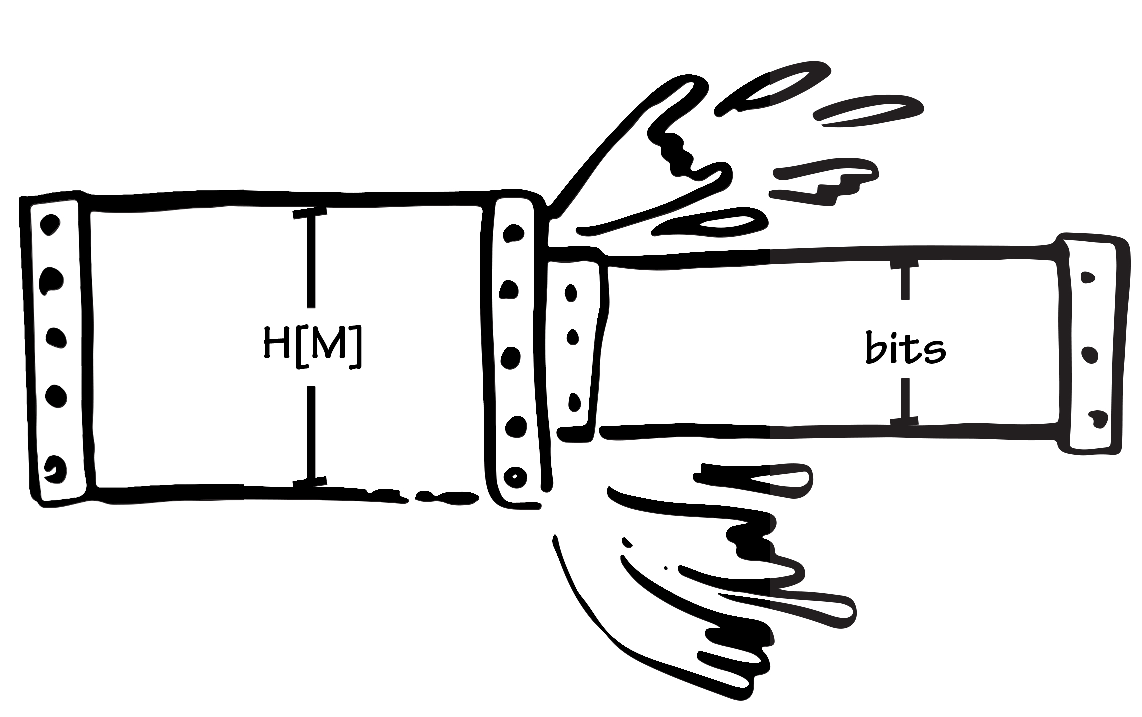
\includegraphics[width=
		\textwidth, left]{tubes5}
		\caption{Loss of information.}\label{fig:information_loss}
	\end{subfigure}
	\begin{subfigure}
		[b]{.4\largefigure} \centering
		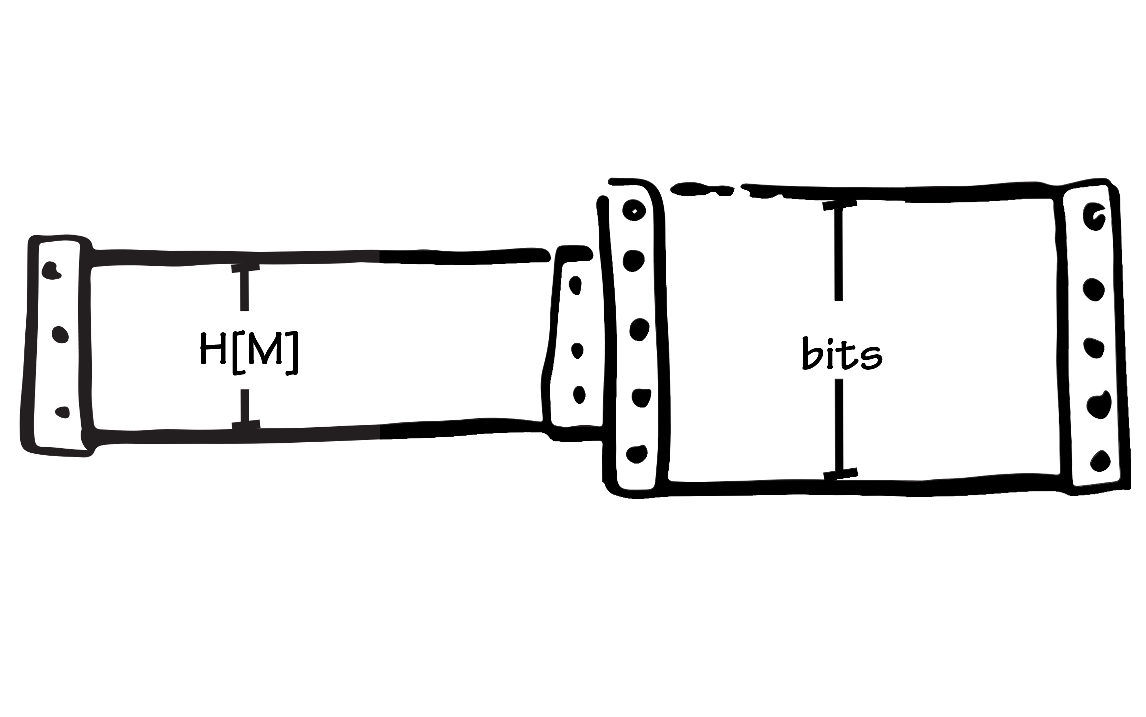
\includegraphics[width=
		\textwidth, left]{tubes6}
		\caption{ Waste of resources (bits).}\label{fig:resource_waste}
\end{subfigure}
\hfill
}
\caption{Entropy of the source vs. coding capacity.}\label{fig:tube}
\end{figure}
Shannon proved a relation between the source's entropy and its optimal encoding (this relation will be shown in \cref{sec:source_encoding_theorem}). The source's entropy is a lower bound on the minimum bits/symbol needed to encode it. The intuition is simple, imagine the Entropy of the source as a ``tube ``(see \cref{fig:tube}). The capacity of the tube is the rate of bits/symbol we expect from the source. The encoder is a connection to the tube.

If we use fewer bits than the entropy to encode it, we are losing information (see \cref{fig:information_loss}). If we use more bits than the entropy, we are wasting resources (see \cref{fig:resource_waste}).
\subsection{An encoding example}
Let us use an example to illustrate better this crucial concept in \ac{IT}\footnote{This example is inspired by~\citeauthor{geron:2018}}. Imagine you are building a weather station that sends the moment weather condition to a distant control room. Also, there are eight weather conditions in which we are interested. In this case, a message is the transmission of one symbol from \(\srcalph\).
\begin{align}
	\srcalph = \{\rw_0, \rw_1, \rw_2, \rw_3, \rw_4, \rw_5, \rw_6, \rw_7\}
\end{align}
\begin{figure}
	[hbt!] \centering
	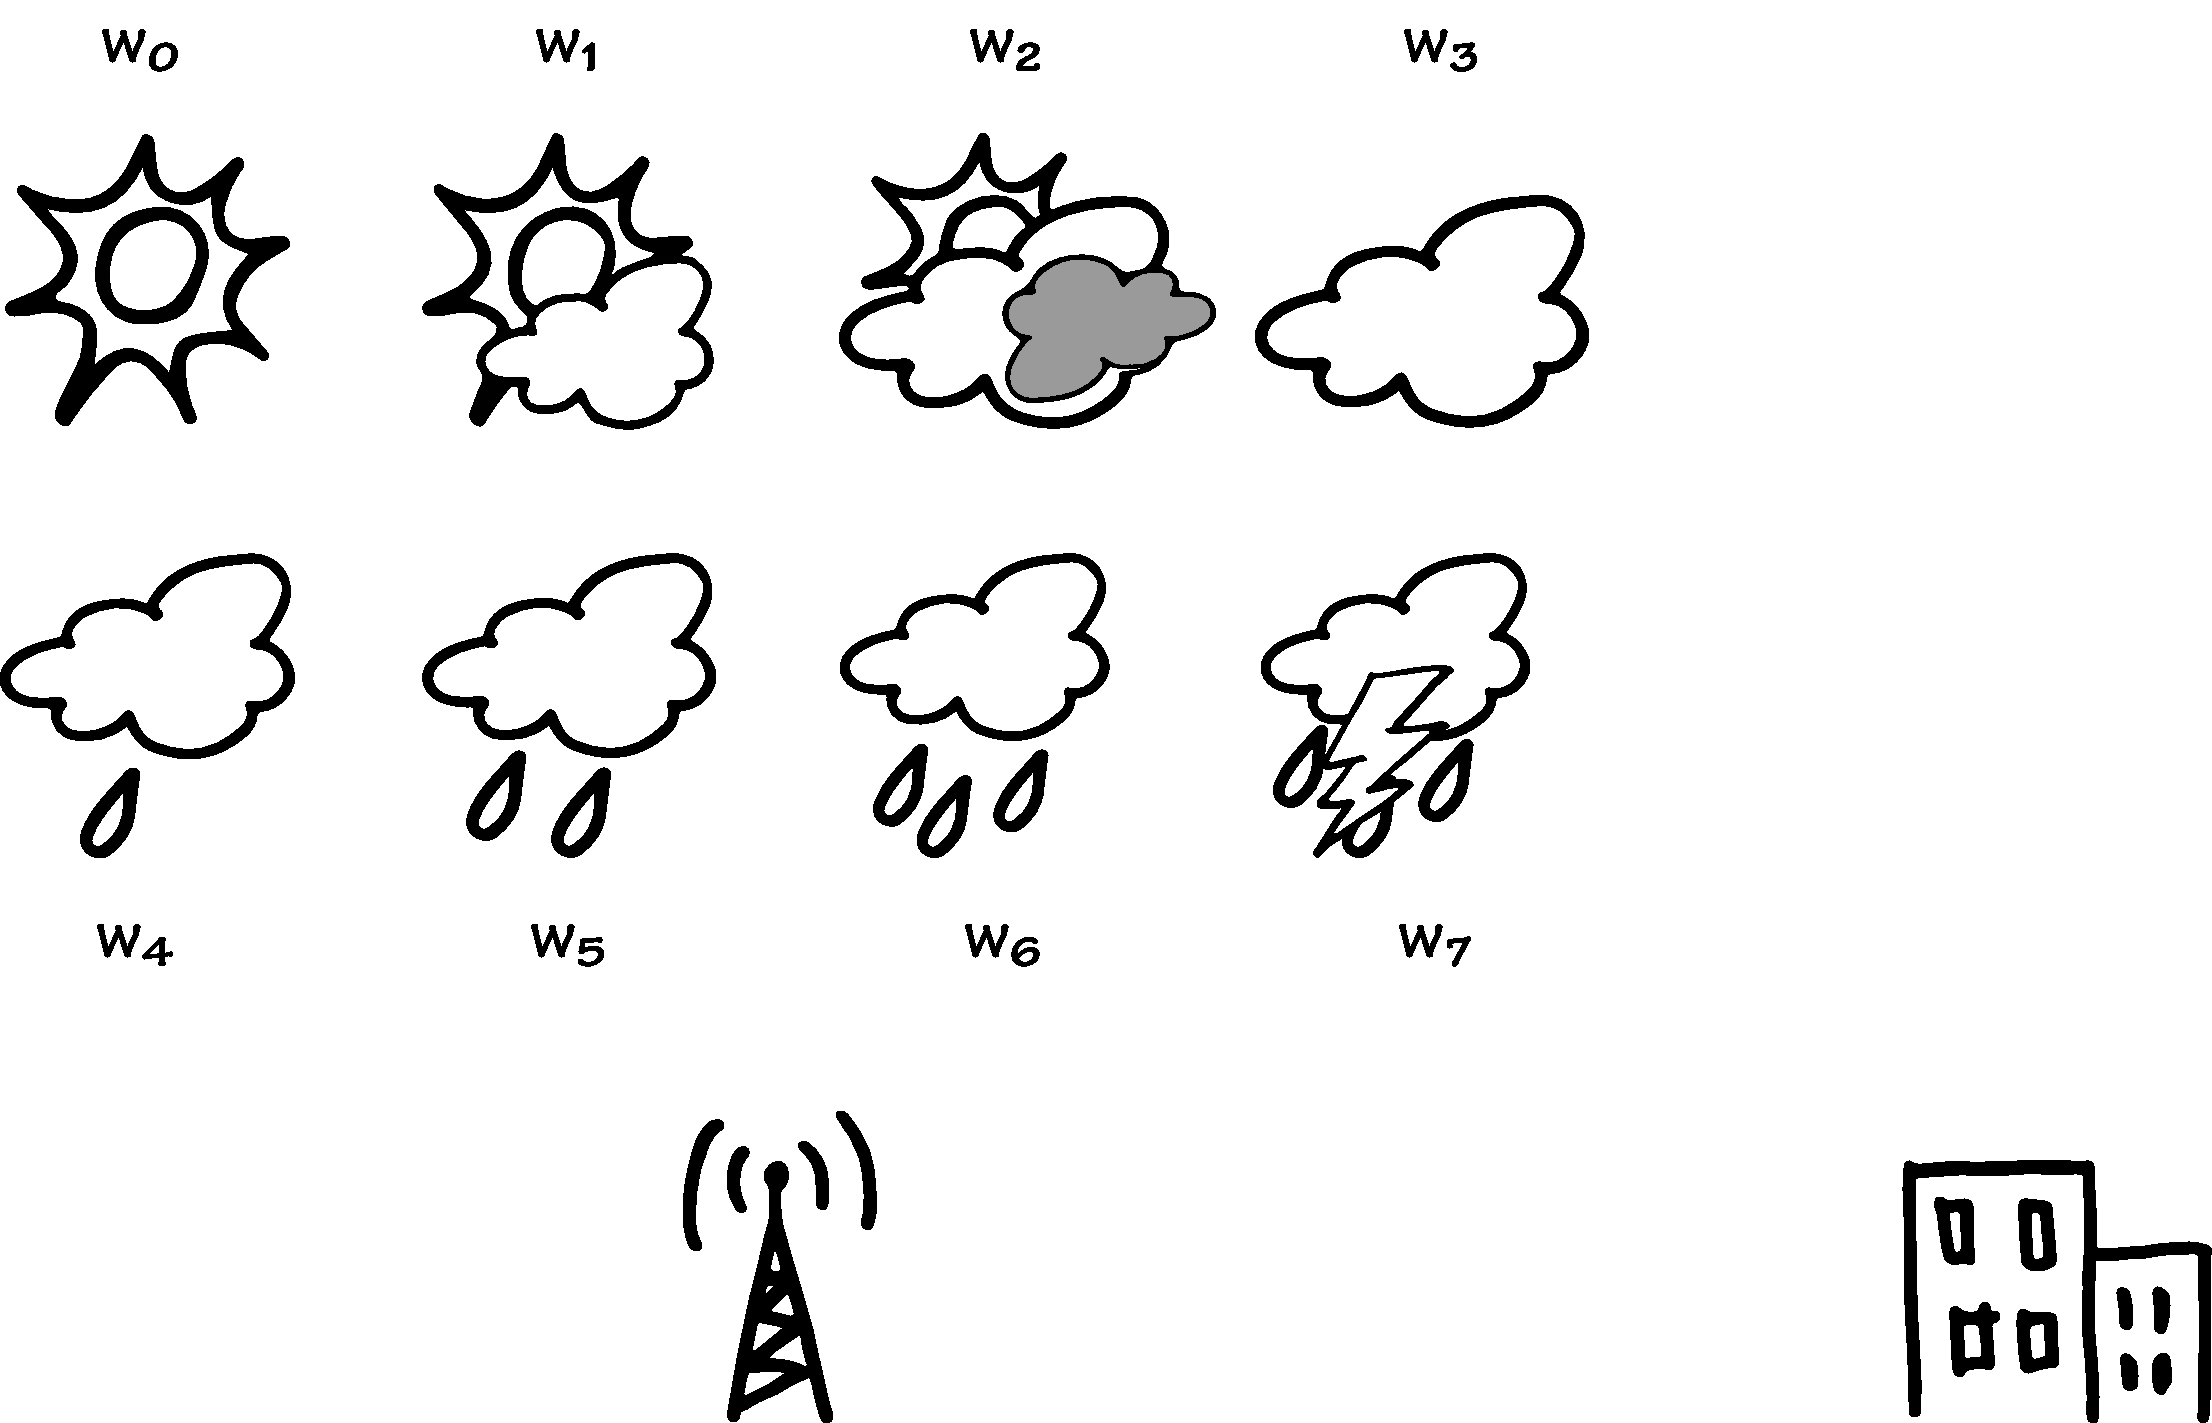
\includegraphics[width=
	\textwidth]{weather_station}
	\caption{A weather station.}\label{fig:weather_station} \end{figure}
How can we encode these weather conditions?

\subsection{Raw bit content} The first idea is to enumerate \(\srcalph\) in binary, using 3 bits/symbol.
\begin{align}
	\encalph = \{&\encsymb_0=000, \encsymb_1=001, \encsymb_2=010, \encsymb_3=011, \nonumber \\
	&\encsymb_4=100, \encsymb_5=101, \encsymb_6=110, \encsymb_7=111\} \label{example_encoding}
\end{align}
\begin{figure}
	[ht!] \centering
	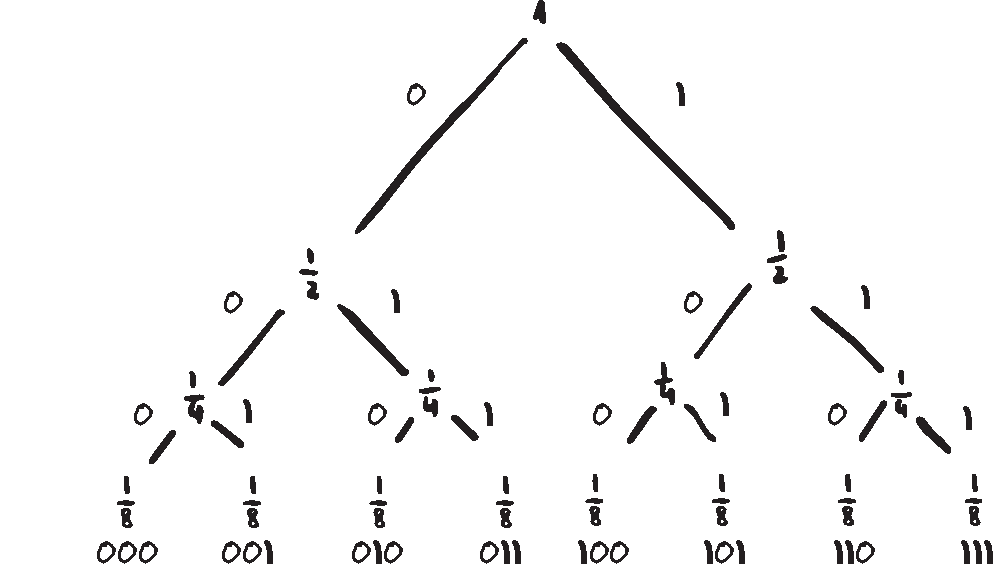
\includegraphics[width=
	\textwidth]{equi_tree}
	\caption{Largest encoding = Maximum entropy.}\label{fig:equi_tree} \end{figure}
This encoding provide a model of the source that has maximum entropy (all outcomes are equiprobable, thus have the same encoding size)\footnote{The probability distribution that produces maximum entropy is the \emph{uniform distribution} (\cref{sec:uniform_distribution})}:
\begin{align}
	p(\encsymb_i)&=\frac{1}{|\encalph|}, \forall i \in [0,7]\\
	H[\enc]&= - \sum^{|\encalph|}\frac{1}{|\encalph|} \log \frac{1}{|\encalph|}\\
	&= \log |\encalph|.
\end{align}
Is this a good encoding?

\subsection{Maximum Entropy Principle}
If all information we have is how many weather conditions are there, the size of the source alphabet, the best model is the one that conveys this information and has maximum Entropy, \ie{}it makes no further assumptions. This maximally entropic model have the worst-case scenario for the average number of questions needed to find out which outcome is the right one:
\begin{align}
	P({\src}) = \{&p_0=\tfrac{1}{8},p_1=\tfrac{1}{8},p_2=\tfrac{1}{8},p_3=\tfrac{1}{8}, \nonumber \\
	&p_4=\tfrac{1}{8},p_5=\tfrac{1}{8},p_6=\tfrac{1}{8},p_7=\tfrac{1}{8}\}
\end{align}

In this case, that encoding (\eqref{example_encoding}) is indeed a good option.
Notice that the encoding process yields a specific distribution \(P(\enc)\), which determines its entropy \(H[\enc]\) and, therefore, how much information per symbol it carries~\cite{stone:2015}. The maximum entropy is obtained with this equiprobable distribution, the \emph{uniform distribution} (\cref{sec:uniform_distribution}).

Let us assume now that another information about the source is given. The weather station is in Atacama, and \(P({\src'}) = \{p_0=75\%,p_1=10\%,p_2=5\%,p_3=1\%, p_4=1\%,p_5=1\%,p_6=1\%,p_7=1\% \}\).
\begin{figure}
	[ht!] \centering
	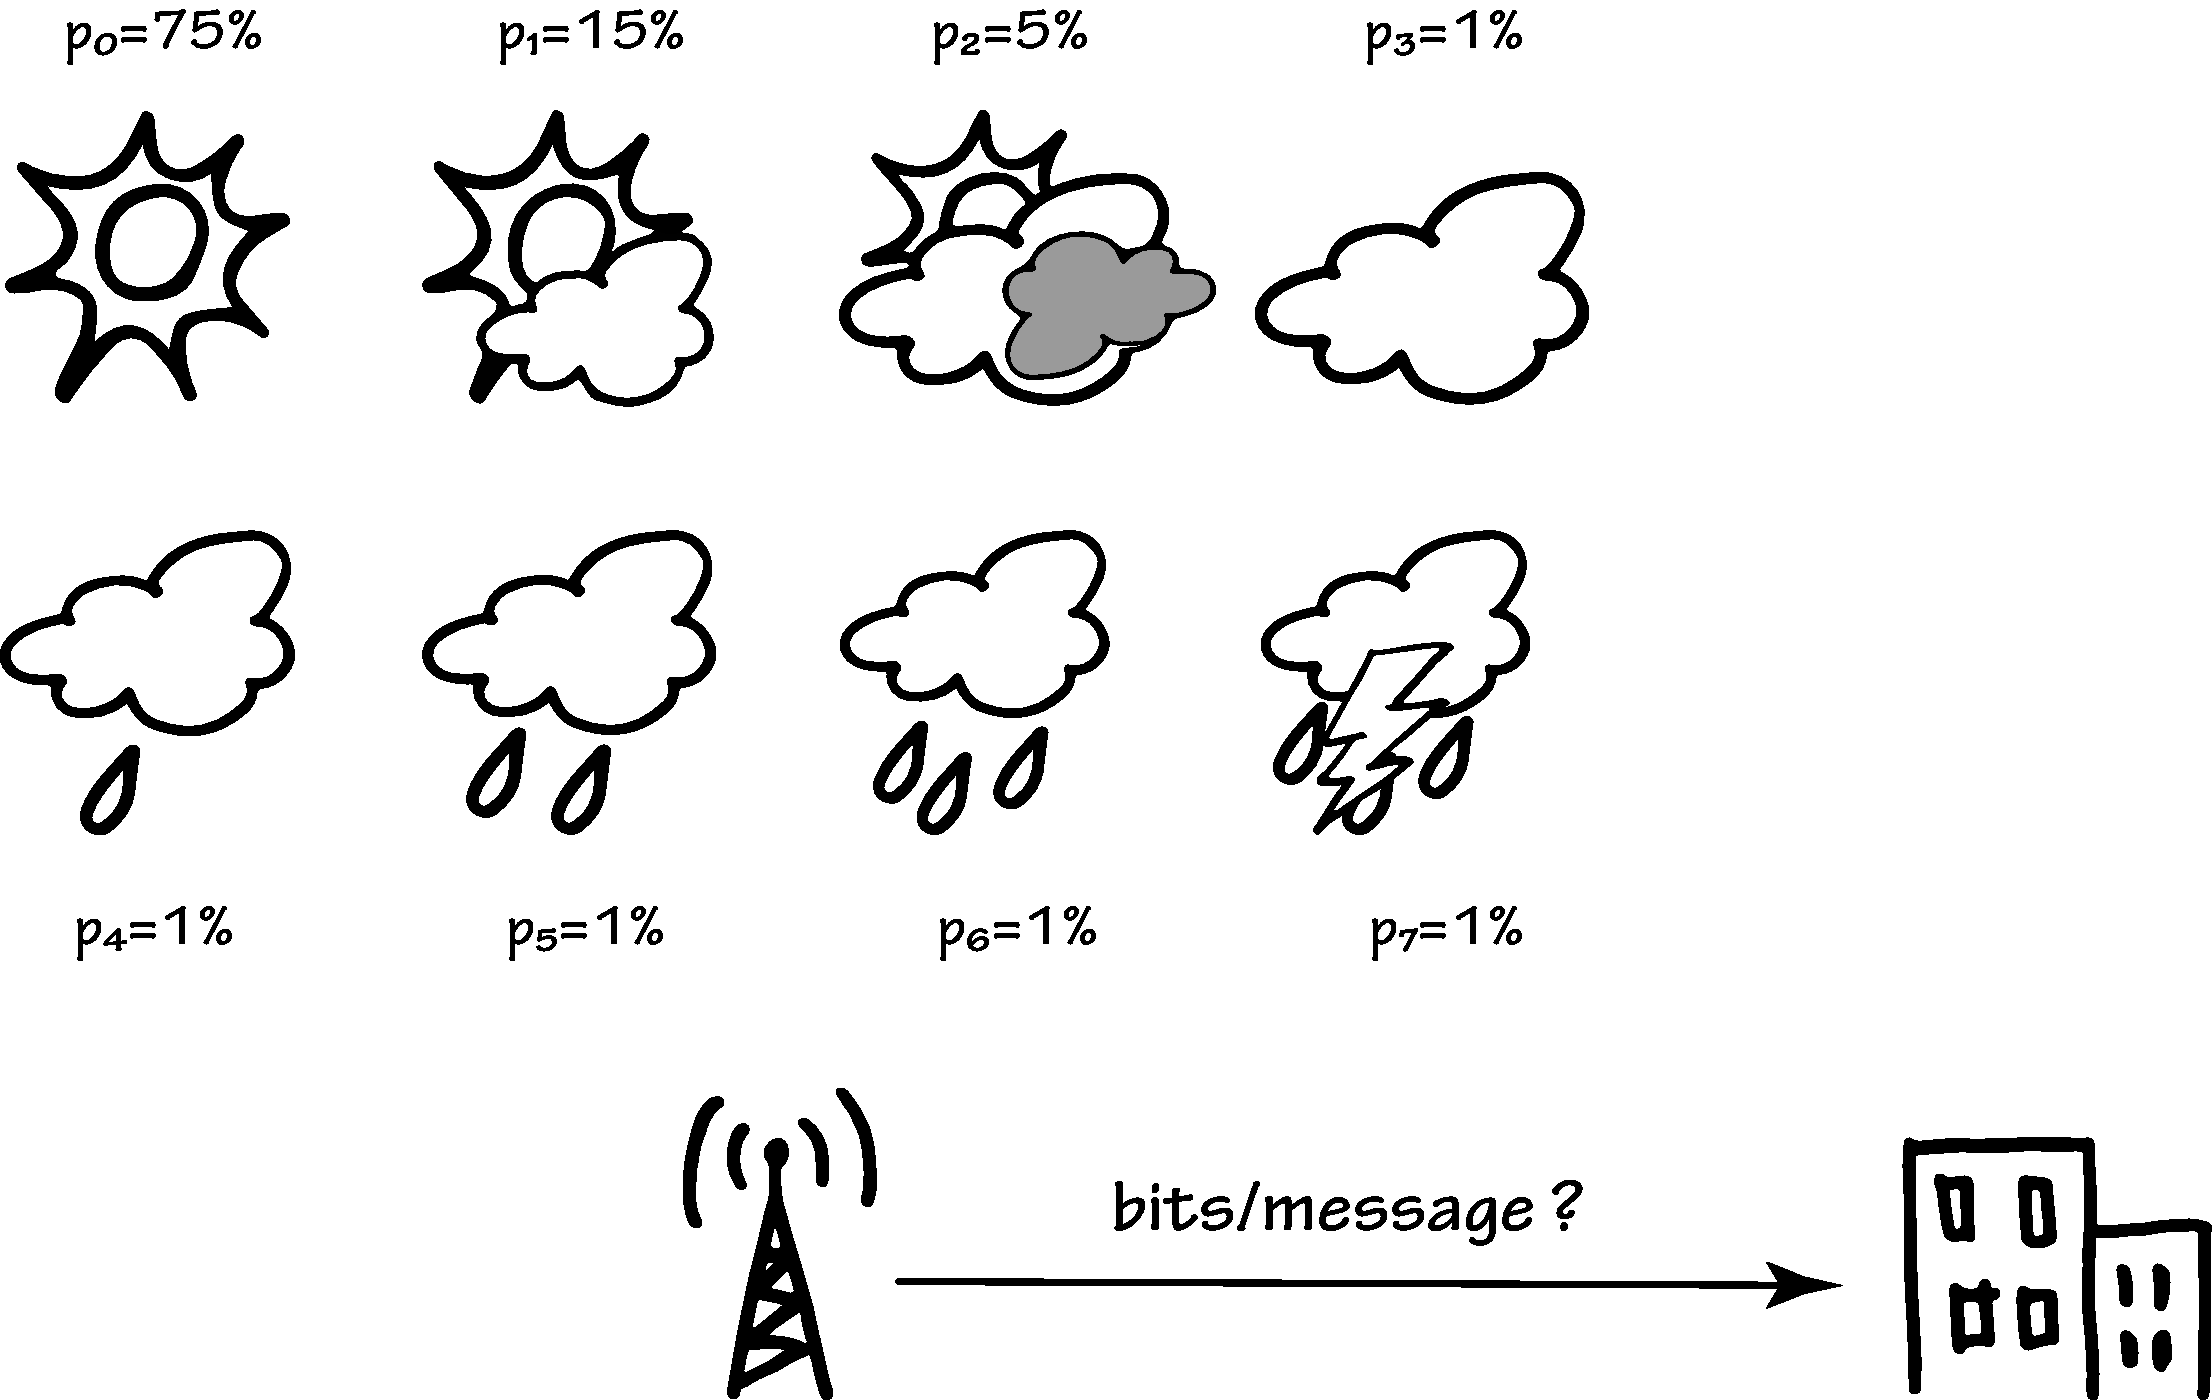
\includegraphics[width=
	\textwidth]{weather_station2}
	\caption{A weather station in Atacama.}\label{fig:atacama} \end{figure}
With this new information about the source. Can we do better? Sure.

First, let us calculate the lower bound (maximum efficiency) of the bits/symbol rate of the source encoding:
\begin{align}
	H[\src']&= 0.75 \log \frac{1}{0.75} + 0.15 \log \frac{1}{0.15} + 0.05 \log \frac{1}{0.05} + 5\biggl(0.01 \log \frac{1}{0.01}\biggr) \nonumber \\
	&\approx 1 \frac{\text{bits}}{\text{symbol}}
\end{align}

We know that theoretically we cannot have an encoding with less than 1 bit/symbol in average. But we can improve from 3 bits/symbol (see \cref{fig:inequi_tree})\footnote{Any distribution that is not uniform will lead to an average tree height that is smaller that the uniform distribution. The uniform distribution is the worst case.}:
\begin{figure}
	[hbt!] \centering
	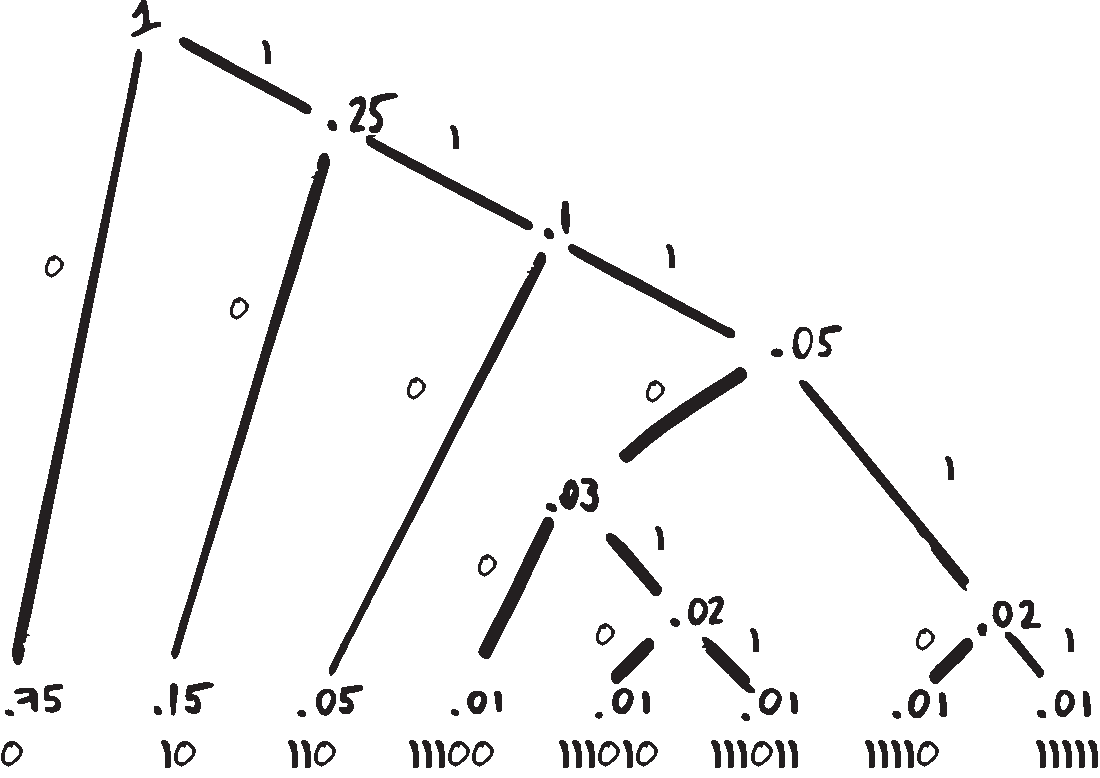
\includegraphics[width=
	.75\textwidth]{ineq_tree}
	\caption{The probability distribution of the source determines an encoding.}\label{fig:inequi_tree} \end{figure}
\begin{align}
	\sA_{\enc'} = \{&\encsymb'_0=0, \encsymb'_1=10, \encsymb'_2=110, \encsymb'_3=11100,\nonumber \\
	&\encsymb'_4=111010, \encsymb'_5=111011, \encsymb'_6=11110, \encsymb'_7=11111\}
\end{align}

The average encoding size per message symbol in \(\enc'\) is:
\begin{align}
	&0.75 \cdot 1 + 0.15 \cdot 2 + 0.05 \cdot 3 + 0.03 \cdot 5 + 0.02 \cdot 6 \nonumber \\
	&\approx 1.5 \frac{\text{ bits}}{\text{symbol}}
\end{align}

\subsection{Cross-Entropy}\label{sec:cross-entropy}
This average encoding size per message symbol has a special name: the Cross-Entropy. It is evident the similarity of the definition of Cross-Entropy and Entropy. If our model \(q\) of the real distribution \(p\) is absolute right, the Cross-Entropy is equal to the Entropy \(H_{p,q}=H_p\). If not (as it is in most cases), \(H_{p,q} > H_p \).

In our Atacama weather station example, the cross-entropy between the real distribution \(p=p(\srcsymb)\) and the encoding distribution \(q=p(\encsymb)\) was 1.5 bits/symbol. So, we can say the efficiency of the encoding \(\enc(\srcsymb)\) is \(\tfrac{\text{information}}{\text{data}} = \tfrac{H[\src]}{H_{p,q}[\src]} = \tfrac{1}{1.5} \approx 67\%\). We calculated  \(H_{p,q}\) knowing the sizes of each possible \(\srcsymb_i\).

Let us use another example, imagine that we transport the weather station from Atacama to London, where the probability distribution of the weather is \(P({\src''}) = \{p_0=5\%,p_1=5\%,p_2=10\%,p_3=15\%, p_4=15\%,p_5=20\%,p_6=20\%,p_7=10\% \} \therefore H[\src'']\approx 2.8\), and keep using the same encoding. It is obvious that the encoding will me much less efficient.
\begin{figure}
	[ht!] \centering
	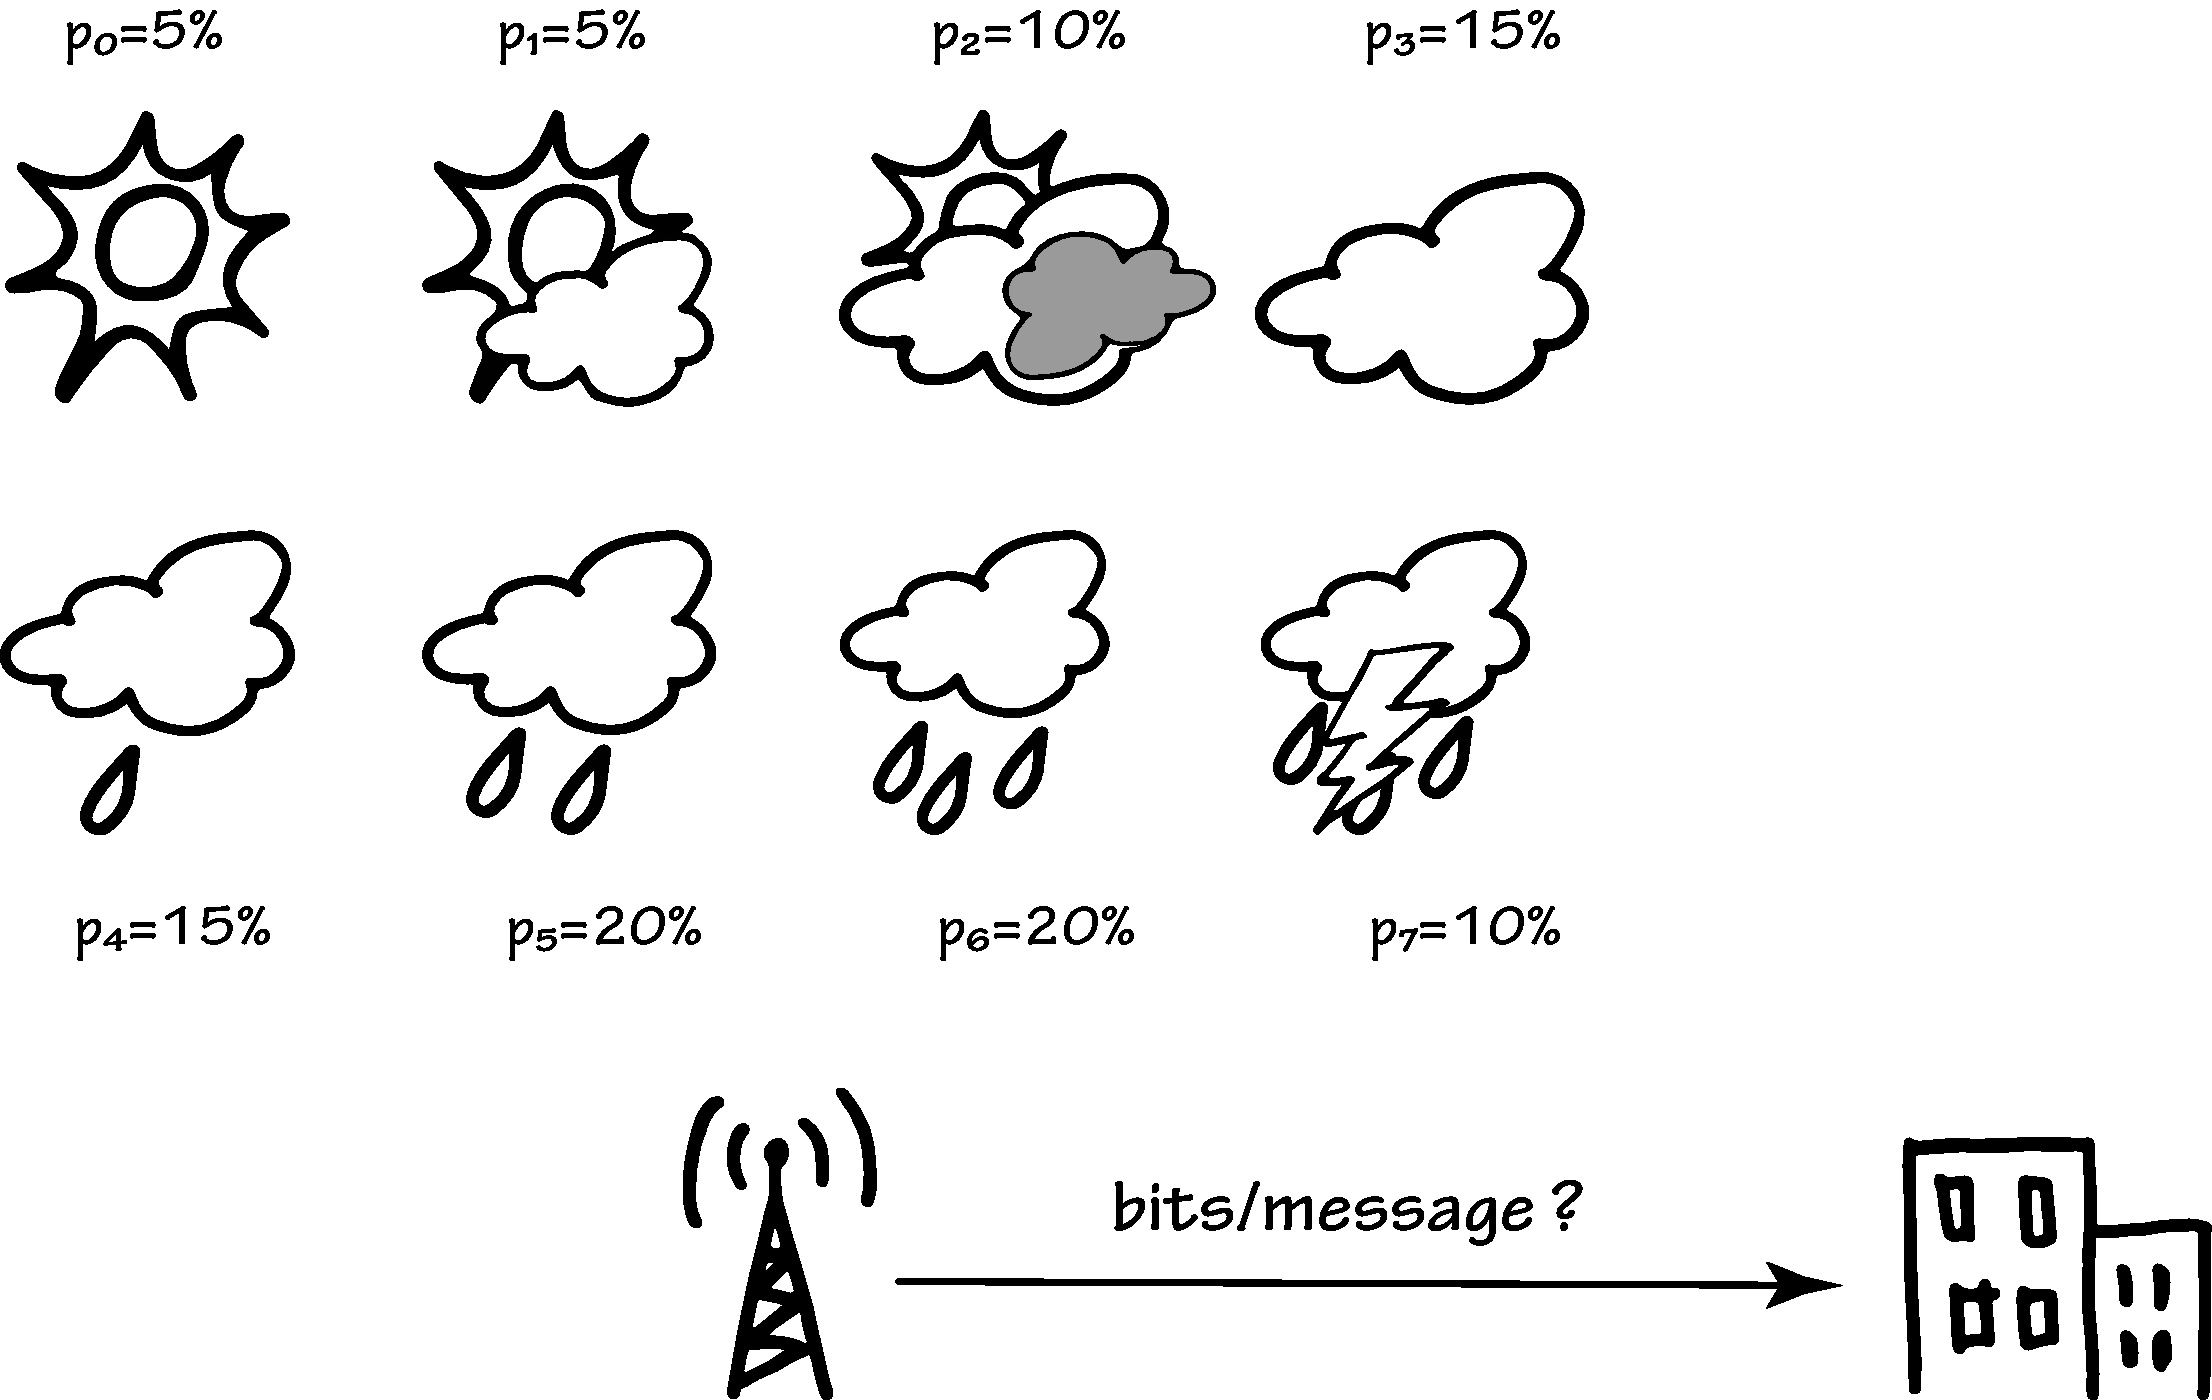
\includegraphics[width=
	\textwidth]{weather_station3}
	\caption{The Atacama's weather station in London.}\label{fig:london} \end{figure}
The average size of a message symbol in this situation is:
\begin{align}
	H_{p,q}[\src''],~ &p = P(\src''), q = P(\enc') \\
	&= 0.05 \cdot 1 + 0.05 \cdot 2 + 0.1 \cdot 3 + 0.45 \cdot 5 + 0.35 \cdot 6 \nonumber \\
	&\approx 4.8 \frac{\text{ bits}}{\text{symbol}}
\end{align}
\begin{definition}
	\textbf{Cross-entropy} is the average number of bits needed to encode data coming from a source \(\src\) with distribution \(p(\srcsymb)\) when using model \(q(\srcsymb)\).
	\begin{align}
		H_{p,q}[\src]=-\sum_{\srcsymb \in \sA_{\src}} p(\srcsymb) \log q(\srcsymb)
	\end{align}
\end{definition}

\subsection{KL Divergence (or Relative Entropy)} The amount by which the Cross-Entropy and the Entropy diverge is the KL Divergence:
\begin{definition}
	The \textbf{relative entropy or Kullback–Leibler divergence} between two probability distributions \(p(\srcsymb)\) and \(q(\srcsymb)\) that are defined over the same alphabet \(\srcalph \) is:
	\begin{align}
		\KL(p||q) = \sum_{\srcsymb} p(\src)~\log \frac{p(\srcsymb)}{q(\srcsymb)}\\
		\KL(p||q) = H_{p,q}[\src] - H_p[\src] \label{eq:KL_decomposition}
	\end{align}
\end{definition}
In our example:
\begin{align}
	\KL(p_{\text{Atacama}}||q_{\text{London}}) = \underbrace{H_{p,q}[\src'']}_{\approx 4.8} - \underbrace{H_p[\src'']}_{\approx 2.8} \approx 2 \frac{\text{bits}}{\text{symbol}}
\end{align}

\subsection{Shannon's source encoding theorem}\label{sec:source_encoding_theorem}
Now that we understand how the source encoding works, let us take a moment to appreciate the geniality of Shannon.  Here, we show how he demonstrated the size of the optimal encoding without ever explaining which encoding is that in the first place.

\begin{theorem}\label{th:source_encoding}
	The optimal binary enconding \(\enc^{k}=(X_1, \cdots, X_k),~ \enc_i \in \{0,1\}\),  of a n-symbols message \(\srcblk=(\src_1, \cdots, \src_n)\), where \(\src_i \in \srcalph\) are i.i.d.\footnote{An \st{obsessive} observant reader may have noticed that we are here considering the source as an i.i.d. stochastic process, instead of a stationay ergodic process.  This is the same proof stated by Shannon in~\cite{shannon:1948} and in several \ac{IT} books (\eg~\cite{cover:2006,mackay:2002}). A proof for ergodic finite alphabet sources can be found in~\cite{mcmillan:1953}.} \(\sim p(\srcsymb)\) has size \(k \approx n H[\src]\) for large \(n\).
\end{theorem}
\begin{proof}
	A one-to-one mapping \(\srcblk \mapsto \enc^{k}\) is invertible. If we enumerate all elements of \(\srcblk\) in binary, we will need \(k\) bits. Thus, with absolute certainty:
	\begin{align}
		k\leq \log \lceil|\srcblk |\rceil = \log \lceil 2^{n \log |\srcalph|}\rceil = n \log |\srcalph|+1~\text{ bits}\label{eq:k_upperbound}
	\end{align}
	Can we do better? We know from statistics that most possible outcomes are unlikely. In other words, there is a small set of very likely outcomes that is most probable. So let us use this property of Nature.
	\begin{figure}
		[ht!] \centering
		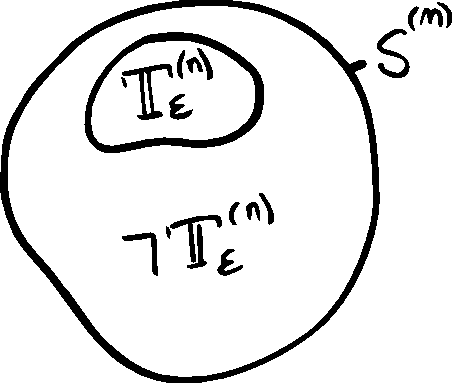
\includegraphics[width=.6\textwidth]{typicalset}
		\caption{The typical set of  sequences \(\srcblk\).}\label{fig:typical_atypical} \end{figure}

	We will divide all sequences \(\srcblk\) into two sets: the typical set (\(\typicalset\)) and its complement, the atypical set (\(\neg~ \typicalset\)), which can be seen in \cref{fig:typical_atypical}.

	\begin{definition}
		The \textbf{typical set} \(\typicalset\) with respect to \(p(\srcsymb)\) is the subset of sequences \(\srcblk=(\src_1,\cdots,\src_n ), \src_i \in \srcalph\), where:
		\begin{align}
			P(\typicalset)=\sum_{\srcblk \in \typicalset} P(\srcblk)> 1-\epsilon, \text{ for sufficiently large }n.\label{typical_set_definition}
		\end{align}
	\end{definition}
	In other words, for a sequence of \(n\) i.i.d random variables \(\src \equiv(\src_1,\cdots,\src_n )\), each drawn from \(p(\srcsymb)\), the outcome \(\vm=(\srcsymb_1, \cdots, \srcsymb_n)\) is almost certain to belong to the typical set \(\typicalset\), if n is large.

	Let us put aside that we do not know the size of the typical set, \(|\typicalset|\).

	We know that:
	\begin{align}
		|\typicalset| &\ll |\neg \typicalset| < |\srcblk |, \\
		P(\typicalset)&\gg P(\neg \typicalset ),\\
		\E(k) &= \lceil P(\typicalset)\log|\typicalset| + P(\neg \typicalset )\log |\neg \typicalset|\rceil.
	\end{align}

	Therefore, from~\eqref{eq:k_upperbound} we can predict that:
	\begin{align}
		\E(k) &\ll  n \log |\srcalph|+1~\text{ bits}
	\end{align}

	Now, we need to find \(|\typicalset|\). For this we will use the \acf{AEP}, formalized in the following Theorem~\cite{cover:2006}:
	\begin{theorem}[\ac{AEP}]\label{th:aep}
		If \(\src_1, \cdots, \src_n\) are i.i.d. from the same \(\sim p(\srcsymb)\), then:
		\begin{align}
			-\frac{1}{n}\log P(\src_1, \cdots, \src_n) \to H[\src] \text{ in probability.}
		\end{align}
	\end{theorem}
	\begin{proof}
		From the theorem definition,  \(\src_i\) are independent. Then from the Product Rule (eq. \ref{eq:Product_Rule}):
		\begin{align}
			- \frac{1}{n} \sum_{i=1}^{n}P(\underbrace{\src_1, \cdots, \src_n}_{\srcblk}) &\overset{\text{~eq.\ref{eq:Product_Rule}}}{=} -\frac{1}{n} \log(\prod_{i=1}^{n} \cancelto{p(\srcsymb)}{P(\src_i))}\\
			&=\frac{1}{n} \sum_{i=1}^{n} -\log p(\srcsymb)
		\end{align}
		From the weak law of large numbers:
		\begin{align}
		 n \to \infty,~\frac{1}{n} \sum_{i=1}^{n}\xi_i \to \mathbb{E}(\xi) \label{eq:law_large_numbers}
		\end{align}
		Therefore, using the fact that a statistic of a random variable is a random variable, let \(\xi=- \log P(\src_i)\)~\cite{cover:2006} and using~\eqref{eq:entropy} and~\eqref{eq:law_large_numbers}:
		\begin{align}
			n \to \infty,& \nonumber\\
			\frac{1}{n} \sum_{i=1}^{n}(- \log P(\src_i))
			&\to \underbrace{\E_p (- \log p(\srcsymb))}_{H[\src]}\\
			\therefore -\frac{1}{n}\log P(\srcblk) &\to H[\src]~\qed
		\end{align}
	\end{proof}
		Now that we proved the \ac{AEP} theorem (Theorem~\ref{th:aep}), let us use it to define \(|\typicalset|\):
		\begin{align}
			-\frac{1}{n} \log P (&\srcblk)\to H[\src] \text{ in probability}\\
			P (&\srcblk) \to 2 ^{-n(H[\src])} \therefore\\
			2 ^{-n(H[\src] + \epsilon)}\leq P (&\srcblk)\leq 2 ^{-n(H[\src] - \epsilon)} \text{ in probability}\label{eq:epsilon}
		\end{align}
		We also now that:
		\begin{align}
			1 &= \sum_{\srcblk} P(\srcblk)\\
			1 &\geq \sum_{\srcblk \in \typicalset}P(\srcblk)\\
			1 &\geq |\typicalset|~ P(\srcblk)
		\end{align}
		From~\eqref{eq:epsilon}:
		\begin{align}
			1 &\geq |\typicalset|~ 2 ^{-n(H[\src] + \epsilon)}\\
			\therefore~ |\typicalset| &\leq 2 ^{n(H[\src] + \epsilon)}\label{eq:typical_upperbound}
		\end{align}
		This upper bound to \(|\typicalset|\) is all we need to prove source coding theorem (Theorem~\ref{th:source_encoding}).
		\begin{align}
			\E(k) &= \lceil P(\typicalset)\log|\typicalset|  \nonumber \\
			&+ \cancelto{\epsilon}{P(\neg \typicalset)} \cancelto{|\srcblk|=n \log |\srcalph|}{\log |\neg \typicalset|} \rceil \\
			&\simeq \lceil (1-\epsilon)\log 2^{n(H[\src]+\epsilon)} + \cancelto{\epsilon' n}{\epsilon n \log |\srcalph|}\rceil\\
			&\simeq \lceil (1-\epsilon)[n(H[\src]+\epsilon)] + \epsilon' n \rceil\\
			&\simeq \lceil n(H[\src]+\epsilon - \epsilon n H[\src] - \epsilon^2) + n (\epsilon')\rceil\\
			&\simeq \lceil n(H[\src]+\cancelto{\epsilon''}{\epsilon - \epsilon H[\src] - \epsilon^2}) +  n (\epsilon')\rceil\\
			&\simeq \lceil n(H[\src]+\epsilon''+\epsilon')\rceil = \lceil n(H[\src]+\varepsilon)\rceil\\
			\therefore \nonumber\\
			\E(k) &\simeq n H[\src] \qedhere
		\end{align}
	\end{proof}
	We proved that the average information per symbol of the coding generated by the optimum encoder has the same average information per symbol as the source, \(H[\src]\frac{\text{bits}}{\text{symbol}}\). Due to this property, it is quite common to talk about \(H[X]\) as the entropy of the source.
\subsection{Typical Set}
In the proof of the source coding theorem, we defined the typical set and discovered some of its properties, but we left one behind. We only needed the upperbound of the \(|\typicalset|\), let us now derive its lowerbound.
From~\eqref{eq:epsilon} and the typical set definition (\eqref{typical_set_definition}):
	\begin{align}
		\sum_{\srcblk \in \typicalset}2^{-n(H[\src]-\epsilon)}&\geq 1 - \epsilon\\
		|\typicalset|2^{-n(H[\src]-\epsilon)}&\geq 1 - \epsilon\\
		|\typicalset|&\geq (1 - \epsilon)2^{n(H[\src]-\epsilon)}\label{eq:typical_lowerbound}
	\end{align}
	Therefore, from~\eqref{eq:typical_lowerbound} and~\eqref{eq:typical_upperbound} we can derive:
\begin{align}
	 (1 - \epsilon)2^{n(H[\src]-\epsilon)} \leq &|\typicalset| \leq 2 ^{n(H[\src]+\epsilon)}\\
	 &|\typicalset| \to 2 ^{nH[\src]}\label{eq:typical_set_size}
\end{align}
With that, we can list some useful properties of \(\typicalset\):
	\begin{enumerate}
		% [i.]
		\item almost all probability is concentrated in the typical set, by definition (\eqref{typical_set_definition});
		\item elements in the typical set are nearly equiprobable,~\eqref{eq:epsilon};
		\item the number of elements in the typical set is nearly \(2^{H[\src]}\),~\eqref{eq:typical_set_size}.
	\end{enumerate}
Going back to the \ac{AEP} theorem (Theorem~\ref{th:aep}):
\begin{align}
	&\frac{1}{n}\log \biggl(\frac{1}{P(\srcblk)}\biggr) &\to H[\src] \nonumber\\
	H[\src] -\epsilon \leq 	&\frac{1}{n}\log \biggl(\frac{1}{P(\srcblk)}\biggr)\leq H[\src] +\epsilon
\end{align}

We can think of the middle term as the Entropy of a sample of size \(n\). Thus a typical sample gives us an amount of information close to the average information from the source, \(H[\src]\)\footnote{This insight reminds us of the sample complexity, which will be discussed in \cref{ch:mlt}}.

\section{The channel: Data transmission} The channel is simply the medium used to transmit the signal \(\encvec\) from the encoder to the decoder. It may be anything from a band of radio frequencies, an electrical wire, a beam of light, or a postal service. As we did before, we can also think the channel as a ``tube'' which carries information (see \cref{fig:tube})\footnote{This definition of a discrete channel covers the deterministic case where \(\decsymb = f(\encsymb)\).\\ In most cases, the usage of a channel is determined by the period in which it is being used.  Thus, some prefer to define the capacity in bits/second.}.

\begin{definition}
	Mathematically, a \textbf{discrete channel} is the conditional probability
	\begin{align}
		p(\decsymb|\encsymb), \decsymb \in \decalph, \encsymb \in \encalph.
	\end{align}
\end{definition}
\subsection{Noiseless Channel Capacity}
\begin{definition}
	The \textbf{operational capacity} of a channel is the maximum rate of bits per usage that the medium is physically capable of transmitting. It is in fact just a number of bits per usage. We can think of it as the maximum entropy it is capable of transmiting in the absence of noise:
	\begin{align}
		\sC_{\text{operational}}= R = \max_{p(\encsymb)} \log |\encalph| \text{ bits/usage}.
	\end{align}
	% In other words, the \emph{operational capacity} \(\sC\) is achieved by the distribution \(p(\encsymb)\) which makes \(H[\enc]\) as large as possible.
\end{definition}

\subsection{The noisy channel}
\begin{figure}
	[hbt!] \centering
	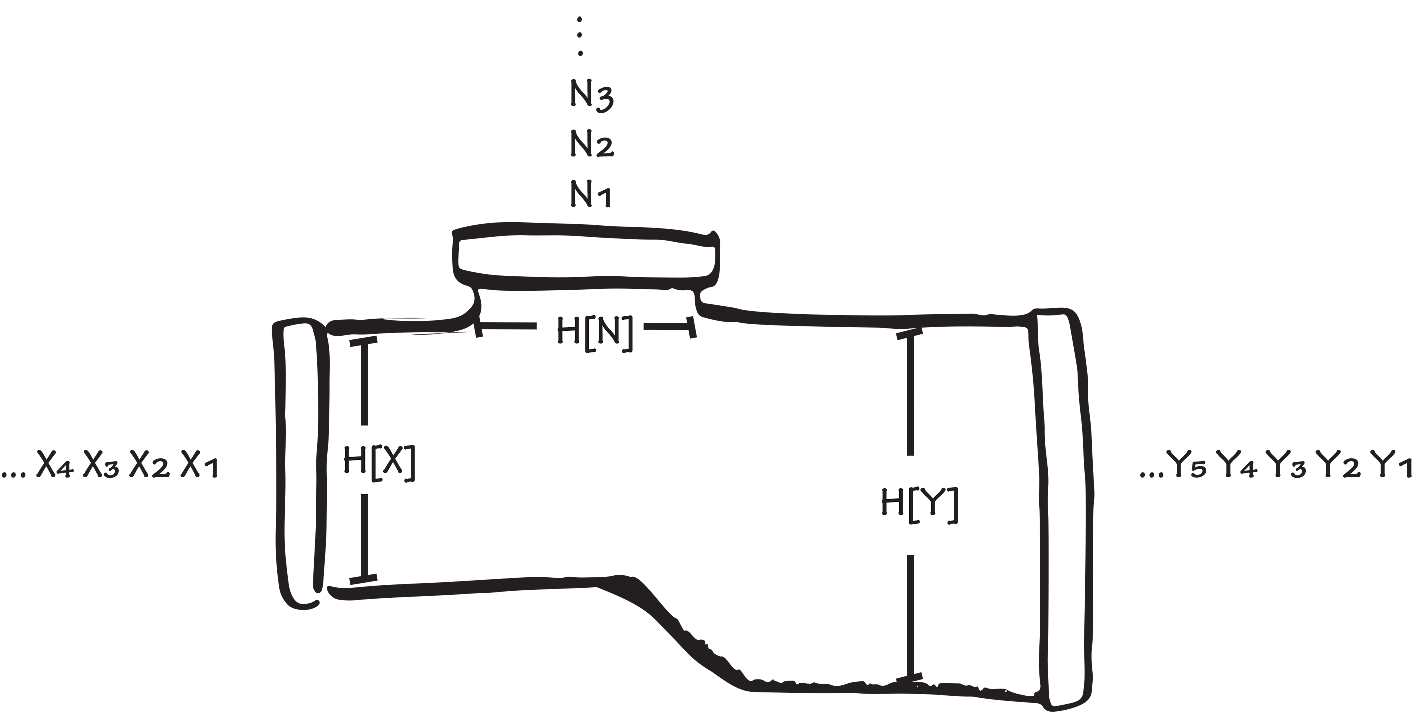
\includegraphics[width=
	\textwidth]{channel}
	\caption{The noisy channel.}
\end{figure}
 All practical communications, however, are noisy~\cite{stone:2015}. Noise reduces the rate at which information can be communicated reliably. Shannon proved that information could be communicated, with arbitrarily small error, at a rate limited only by the channel capacity.

 To understand how noise affects the channel capacity, we need to understand the concepts of \textbf{conditional entropy}, \textbf{joint entropy} and \textbf{mutual information}.
\subsection{Conditional Entropy} The residual uncertainty we have about a random variable \(\dec\), given that we already know the outcome of another random variable \(\enc\) is the \textbf{conditional entropy}:
\begin{definition}
	The \textbf{conditional entropy} or \textbf{equivocation} \(H[\enc|\dec]\) of \(\enc\) given \(\dec\) is:
	\begin{align}
		H[\enc|\dec] &\eqdef \sum_{\decsymb \in \decalph} p(\decsymb) \left[ \sum_{\encsymb \in \encalph} p(\encsymb|\decsymb) \log \frac{1}{p(\encsymb|\decsymb)}\right]\\
		&=- \sum_{\encsymb\decsymb \in \encalph\decalph} p(\encsymb,\decsymb) \log p(\encsymb|\decsymb)
	\end{align}
\end{definition}
% \paragraph{chain rule} From the Product Rule of probabilities (\eqref{eq:Product_Rule}), we have:
% \begin{align}
% 	\log \frac{1}{p(x,y)} = \log \frac{1}{p(x)+ \log \frac{1}{p(y)}}\\
% 	\therefore H[\enc,\dec]=H[\enc]+H[\dec|\enc]
% \end{align}
\subsection{Joint Entropy}
We have defined the entropy of a single random variable in~\eqref{eq:entropy}. Now, we extend the definition to a pair of random variables. As the pair can be seen as a single vector-valued random variable, there is nothing new in this definition~\cite[p.15]{cover:2006}.
\begin{definition}
	The \textbf{joint entropy} \(H[\rvX, \rvY]\) of a pair of discrete random variables \((\rvX, \rvY)\) with joint distribution \(p (x, y)\) is defined as:
	\begin{align}
		H [X,Y] &\triangleq -\E \log P(\rvX, \rvY) \\
		&= - \sum_{\encsymb \in \sA_x} \sum_{\decsymb \in \sA_y} p(\encsymb,\decsymb) \log p(\encsymb,\decsymb).
	\label{eq:joint_entropy} \end{align}
\end{definition}
\subsection{Mutual Information}
\begin{definition}\label{def_mutual_information}
	The \textbf{mutual information} \(I[\enc;\dec]\) between two variables, such as a channel input \(\enc\) and output \(\dec\), is the amount of information obtained about one random variable through observing the other random variable.
	\begin{align}
		I[\enc;\dec] &= \sum_i \sum_j p(\encsymb_i, \decsymb_j) \log \frac{p(\encsymb_i, \decsymb_j)}{p(\encsymb_i) p(\decsymb_j)} \text{ bits} \label{eq:mutual_information}\\
		&= H[\enc] - H[\enc|\dec]\\
		&= H[\dec] - H[\dec|\enc]\\
		&= H[\enc] + H[\dec] - H[\enc, \dec]\\
		&= H[\enc, \dec] - [H[\enc|\dec] + H[\dec|\enc]] \text{ bits}
	\end{align}
\end{definition}
\begin{figure}
	[hbt!] \centering
	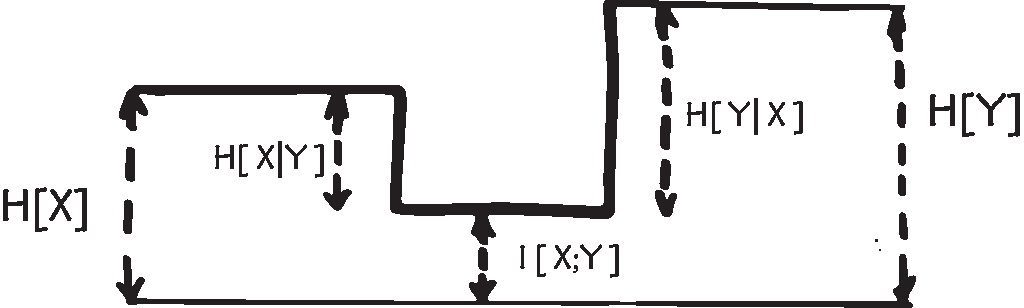
\includegraphics[width=\textwidth]{mutual}
	\caption{Relationship between information measures in a channel.}\label{fig:mutual}
\end{figure}
For a visual understanding of this measures, see \cref{fig:mutual}.
The mutual information can also be seen as a measure of the mutual dependence between the two variables, as the mutual information is the same as the Kullback–Leibler divergence between the joint distribution and the product of the variables marginal distributions:
\begin{align}
	I[\enc;\dec] = \KL(p(\encsymb, \decsymb)||p(\encsymb)p(\decsymb)) .
\end{align}

\subsection{Data Processing Inequality}
We cannot increase information by applying a deterministic function to the data, nor decrease information if the deterministic function is invertible.

\begin{theorem}
	[DPI\footnote{We refer to~\cite[th.2.8.1]{cover:2006} for a proof}] Let three random variables form the Markov chain \(\rvX \rightarrow \rvY \rightarrow \rvZ\), implying:
	\begin{align}
		p(\rx,\ry,\rz)=p(\rx)p(\ry|\rx)p(\rz|\ry).
	\end{align}
	No processing of \(\rvY\), deterministic or random, can increase the information that \(\rvY\) contains about $\enc$:
	\begin{align}
		I[\rvX;\rvY] \geqslant I[\rvX;\rvZ]
	\end{align}
\end{theorem}
\begin{theorem}
	[Reparemetrisation invariance] $I[\rvX;\rvY]\geqslant I[\rvX;g(\rvY)]$: functions of the data $\rvY$ cannot increase the information about $\rvX$.\label{th:reparemetrisation_invariance}
\end{theorem}
\begin{proof}
	\(\rvX \rightarrow \rvY \rightarrow \rvZ\) form a Markov Chain	where $\rvZ=g(\rvY) \therefore I[\rvX;g(\rvY)]=I[\rvX;\rvZ]$. By DPI:\@
	\begin{align}
		I[\rvX;\rvY] \geqslant I[\rvX;\rvZ]\\
		I[\rvX;\rvY] \geqslant I[\rvX;g(\rvY)]
	\end{align}
\end{proof}



\subsection{Noisy channel capacity}
Given that in a noise channel \(\dec = \enc + \noise \), where \(\noise\) is the noise in the channel, from the mutual information definition:
\begin{align}
	I[\enc;\dec]&=H[\dec] - H[\dec|\enc]\\
	&=H[\dec] - H[(\enc + \noise)|\enc].
\end{align}
If $\enc$ is known, the uncertainty from $\enc$ is none:
\begin{align}
	I[\enc;\dec]&=H[\dec] - H[\noise|\enc]
\end{align}
By definition, $\noise$ and $\enc$ are independent, therefore:
\begin{align}
	I[\enc;\dec]&=H[\dec] - H[\noise]\\
	\therefore H[\dec|\enc] &= H[\noise]
\end{align}
% The kind of channel that we are interested in is called an addictive channel, where:
% \begin{align}
% 	\dec &= \enc + \eta \\
% 	H[\dec]&= I[\enc;\dec] + H[\eta]\\
% 	&= I[\enc;\dec] + H[\dec|\enc]
% \end{align}

\begin{definition}
	The \textbf{information capacity} or \emph{effective capacity} of a noisy channel is defined as:
	\begin{align}
		C &= \max_{p(x)} I[\enc,\dec]\\
		&=\max_{p(x)} (H[\dec] - H[\dec|\enc]) \text{ bits/usage.}\\
		&=\max_{p(x)} (H[\enc] - H[\enc|\dec]) \text{ bits/usage}.
	\end{align}
\end{definition}
The information capacity can be derived theorem from Shannon's noisy channel theorem (\ref{noisy_channel_theorem}). Notice that when there is no noise, the definition corresponds to the \emph{operational capacity} definition.

% There is a duality between compression and transmission~\cite{cover:2006}. In compression we remove redundancy to obtain the smallest representation of the message, whereas in transmission we add redundancy in a controlled fashion in order to be able to recover from errors caused by noise in the channel.
\section{The decoder}
The decoder capability of reconstructing the message from the encoded data despite the channel noise is a direct consequence of Shannon's second theorem:

\subsection{Shannon's noisy channel theorem}\label{noisy_channel_theorem}
In his second and, perhaps, most crucial theorem, Shannon proved that, provided \(H[\enc]\leq C\), the average error (\(\epsilon\)), when averaged over all possible encoders, approaches to zero (\(\epsilon \to 0\)) as the length of the input \(\encvec\) increases. Therefore, there must exist at least one encoder that produces an error as small as \(\epsilon\).

Once again, Shannon proved with a counterintuitive argument. He demonstrates there is an encoder that produces an arbitrarily small error without showing how to find this encoder.

Instead of proving the theorem (for which we refer to~\citeauthor{mackay:2002} and~\citeauthor{cover:2006}), let us give an intuitive preview of the proof.

Consider \(n\) uses of the channel as our block usage. There are \(|\encalph|^n\) possible inputs \(\encvec\) and \(|\decalph|^n\) possible outputs \(\decvec\) in the block usage. We want to prove that for any \(\decvec\), it is possible to derive an unique message that generated it.

If \(n\) is large, any particular \(\encvec \in \enc^n\) is very likely to produce an output in a small subspace of the output alphabet, the typical output set, given \(\encvec\). So, it is possible to find a non-confusable subset of the input sequences that produce disjoint output sequences.
% \begin{figure}
% 	[ht!] \centering
% 	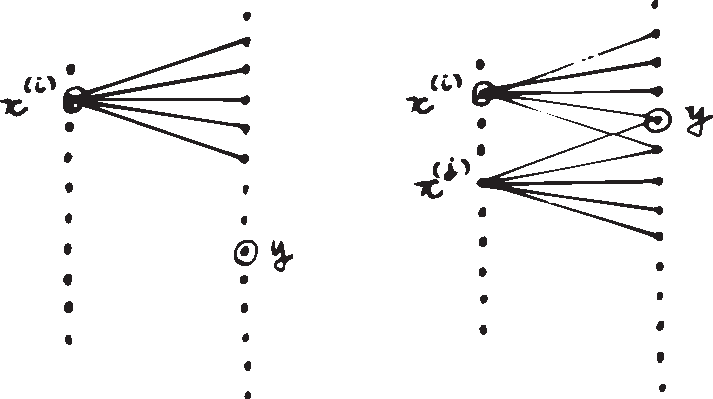
\includegraphics[width=.7\textwidth]{fanchart_2}
% 	\caption{Disjoint output sequences.}\label{fig:disjoint_sequences} \end{figure}
\begin{figure}
	[ht!] \centering
	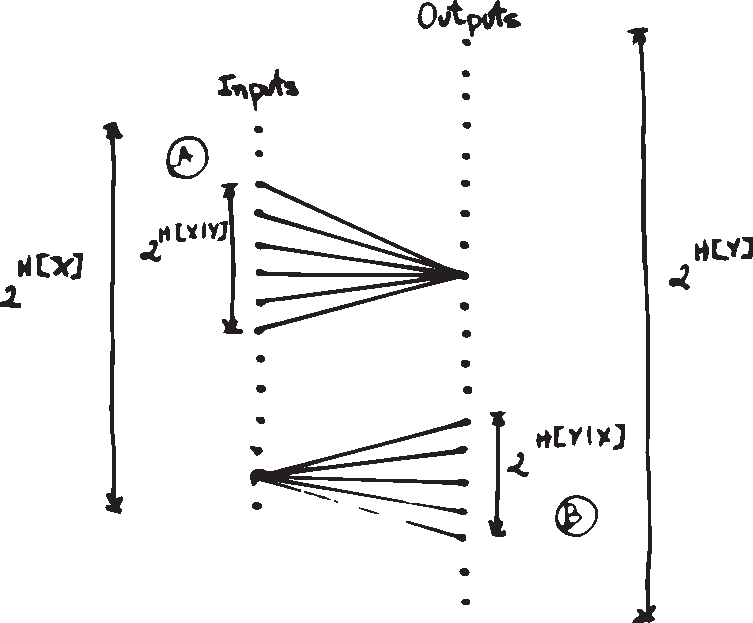
\includegraphics[width=.7\textwidth]{fanchart_1}
	\caption{The need to restrict to the subset of typical inputs and its implications.}\label{fig:fan}
\end{figure}
Take \(\encvec \sim p(\enc^n)\). Recall the source coding theorem (Theorem~\ref{th:source_encoding}), the total number of typical output sequences \(\decvec\) is \(2^{nH[\dec]}\) (see \cref{fig:fan} (B)), all sequences being almost equiprobable. For any sequence \(\encvec\), there are about \(2^{nH[\dec|\enc]}\) probable sequences (see \cref{fig:fan} (A)).

Now we restric ouselves to the subset of the typical inputs such that the correponding typical output sets are disjoint. We can expect the number of non-confusable inputs to be:
\begin{align}
	\leq \frac{2^{nH[\dec]}}{2^{nH[\dec|\enc]}}=2^{n(H[\dec]-H[\dec|\enc])}=2^{nI[\enc;\dec]}
\end{align}

The maximum value of this bound is achieved by the process \(\enc\) that maximises \(I[X;Y]\). Therefore, \(n \max_{p(\encsymb)}I[X;Y]\) is the maximum amount of bits that can be transmitted in \(n\) usages of the channel, which proves the first law of information (see \cref{shannon_laws}):
\begin{align}
	C\text{\tiny{noisy channel}} &= \max_{p(x)} I[\enc,\dec]\label{eq:shannon_1st_law} .
\end{align}

We can rewrite~\eqref{eq:shannon_1st_law} as:
\begin{align}
	C\text{\tiny{noisy channel}} &= \max_{p(x)} (H[\enc]-H[\noise])\label{eq:2nd_law} ,
\end{align}
which states that noise reduces channel capacity. So, this is also a proof for the second law of information (\cref{shannon_laws}).

%
% \subsection{Compression and complexity}
% %


\section{Beyond Shannon's Information}
\subsection{Algorithmic information (Kolmogorov-Chaitin complexity)}
Developed independently by Chaitin, Solomonoff, and Kolmogorov in the 1960s, \emph{algorithmic information} (most commonly known as Kolmogorov complexity) of an object (\eg a message) is the length of the shortest program capable of producing the object as an output\cite{stone:2015}.

For example, in this definition the string 'T6ucFndKEjTyqIGYuXUKqI6fJ6HBRL' is more complex than  'abcabcabcabcabcabcabcabcabcabc'. In python:
\begin{lstlisting}
	"T6ucFndKEjTyqIGYuXUKqI6fJ6HBRL"
\end{lstlisting}
versus
\begin{lstlisting}
	"abc"*10
\end{lstlisting}
If the object is compressable (shorter program), it has more regularity. Thus, there is a relation between complexity and compressibility.
\subsection{Fisher Information}
Let $P_{\theta}$ denote a family of parametric distributions on a space $\XX$ with probability mass or density function given by $p_{\theta}$.

\begin{definition}[Fisher information] The Fisher information $I_{\rvX}(\theta)$ of a random variable $\rvX$ w.r.t. the parameter $\theta$ is the matrix:
	\begin{align}
		[I_{\rvX}(\theta)]_{ij} &:= \E_{\theta} \left[ \nabla_{\theta_i} \log p_{\theta}(\rvX) \cdot  \nabla_{\theta_j} \log p_{\theta}(\rvX)^\top \right] \\
		&= \E_{\theta}\left[ \frac{\partial \ell}{\partial \theta_i} \cdot \frac{\partial \ell}{\partial \theta_j}^\top \right],
	\end{align}
	where $\ell(\rx|\theta)= \log p(\rx|\theta)$ is often called the score function.
\end{definition}
The Fisher information measures the overall sensitivity of the functional relationship $p$ to changes of $\theta$ by weighting the sensitivity at each potential outcome $\rx$ w.r.t $p_{\theta}(\rx)$\cite{maarten:2017}

A common simplification of the Fisher Information Matrix (FIM) is to reduce it to the diagonal:
\begin{align}
	[I_{\rvX}(\theta)]_{i} &:= \E_{\theta} \left[ \nabla_{\theta_i} \log p_{\theta}(\rvX)^2 \right]
\end{align}
\subsection{Shannon vs. Fisher Information}
By using \eqref{eq:ExKL}, \eqref{eq:new_lagrangian} can be rewritten as:
\begin{align*}
  \boldsymbol{\LL(W) = H_{p,q}(D|W) +\beta \KL{\underbrace{q(W|D)}_{\text{training output}}}{\underbrace{p(W)}_{\text{fixed prior}}}}
\end{align*}

In other words, $I(W;D)$ is the divergence of the conditional model distribution $q(W|D)$ and the expected prior averaging all datasets. If, instead, we assume an isotropic gaussian\footnote{An isotropic gaussian is one where the covariance matrix is represented by $\Sigma=\lambda^2 I$.} as the prior, the information in the weights when $W_*$ is minimal, is given by:
\begin{align*}
  \KL{q(W|D)}{p(W)}=\frac{1}{2} \Bigg(\log |F m|+\cancel{\log \lambda^2I} + \cancel{\frac{W_*^2}{\lambda^2I}} \Bigg),
\end{align*}
where the canceled terms are the ones that do not depend on $q(W|D)$ and can be ignored, $\log |F|$ is the log-determinant of Fisher Information Matrix of the weights and $m$ is the number of samples in the dataset.

This is quite interesting as it gives us an analytical and fast calculation of a  bound to $I(W;D)$:
\begin{align}
I(T;X) \leq I(D;W) \leq \log |F(W^*)| \label{bounds}
\end{align}
\section{Connections to Bayesian Inference}
There are countless problems in Science which require that given a limited dataset, preferences be assigned to alternative hypothesis of different complexities. The \textbf{Occam's razor} is the principle that states preference for simple theories. Despite the fact it is often advocated for aesthetic reasons, \citeauthor{mackay:2002} gave a Bayesian explanation for its empirical success that does not depend on any bias towards beauty\cite{mackay:2002}.

Consider the evaluation of the plausability of two alternative theories $\HH_1$ and $\HH_2$, in the light of given evidence ($C$ data). Complex models are capable of making a greater variety of predictions. So, if $\HH_2$ is more complex, it must spread its predictive capability more thinly over the data space $\DD$ than $\HH_1$. Thus, where the gathered data $C$ are compatible with both theories, the simpler $\HH_1$ will be more probable than $\HH_2$ (\cref{modelcomparison}).
\begin{figure}[hbt!]
	\centering
	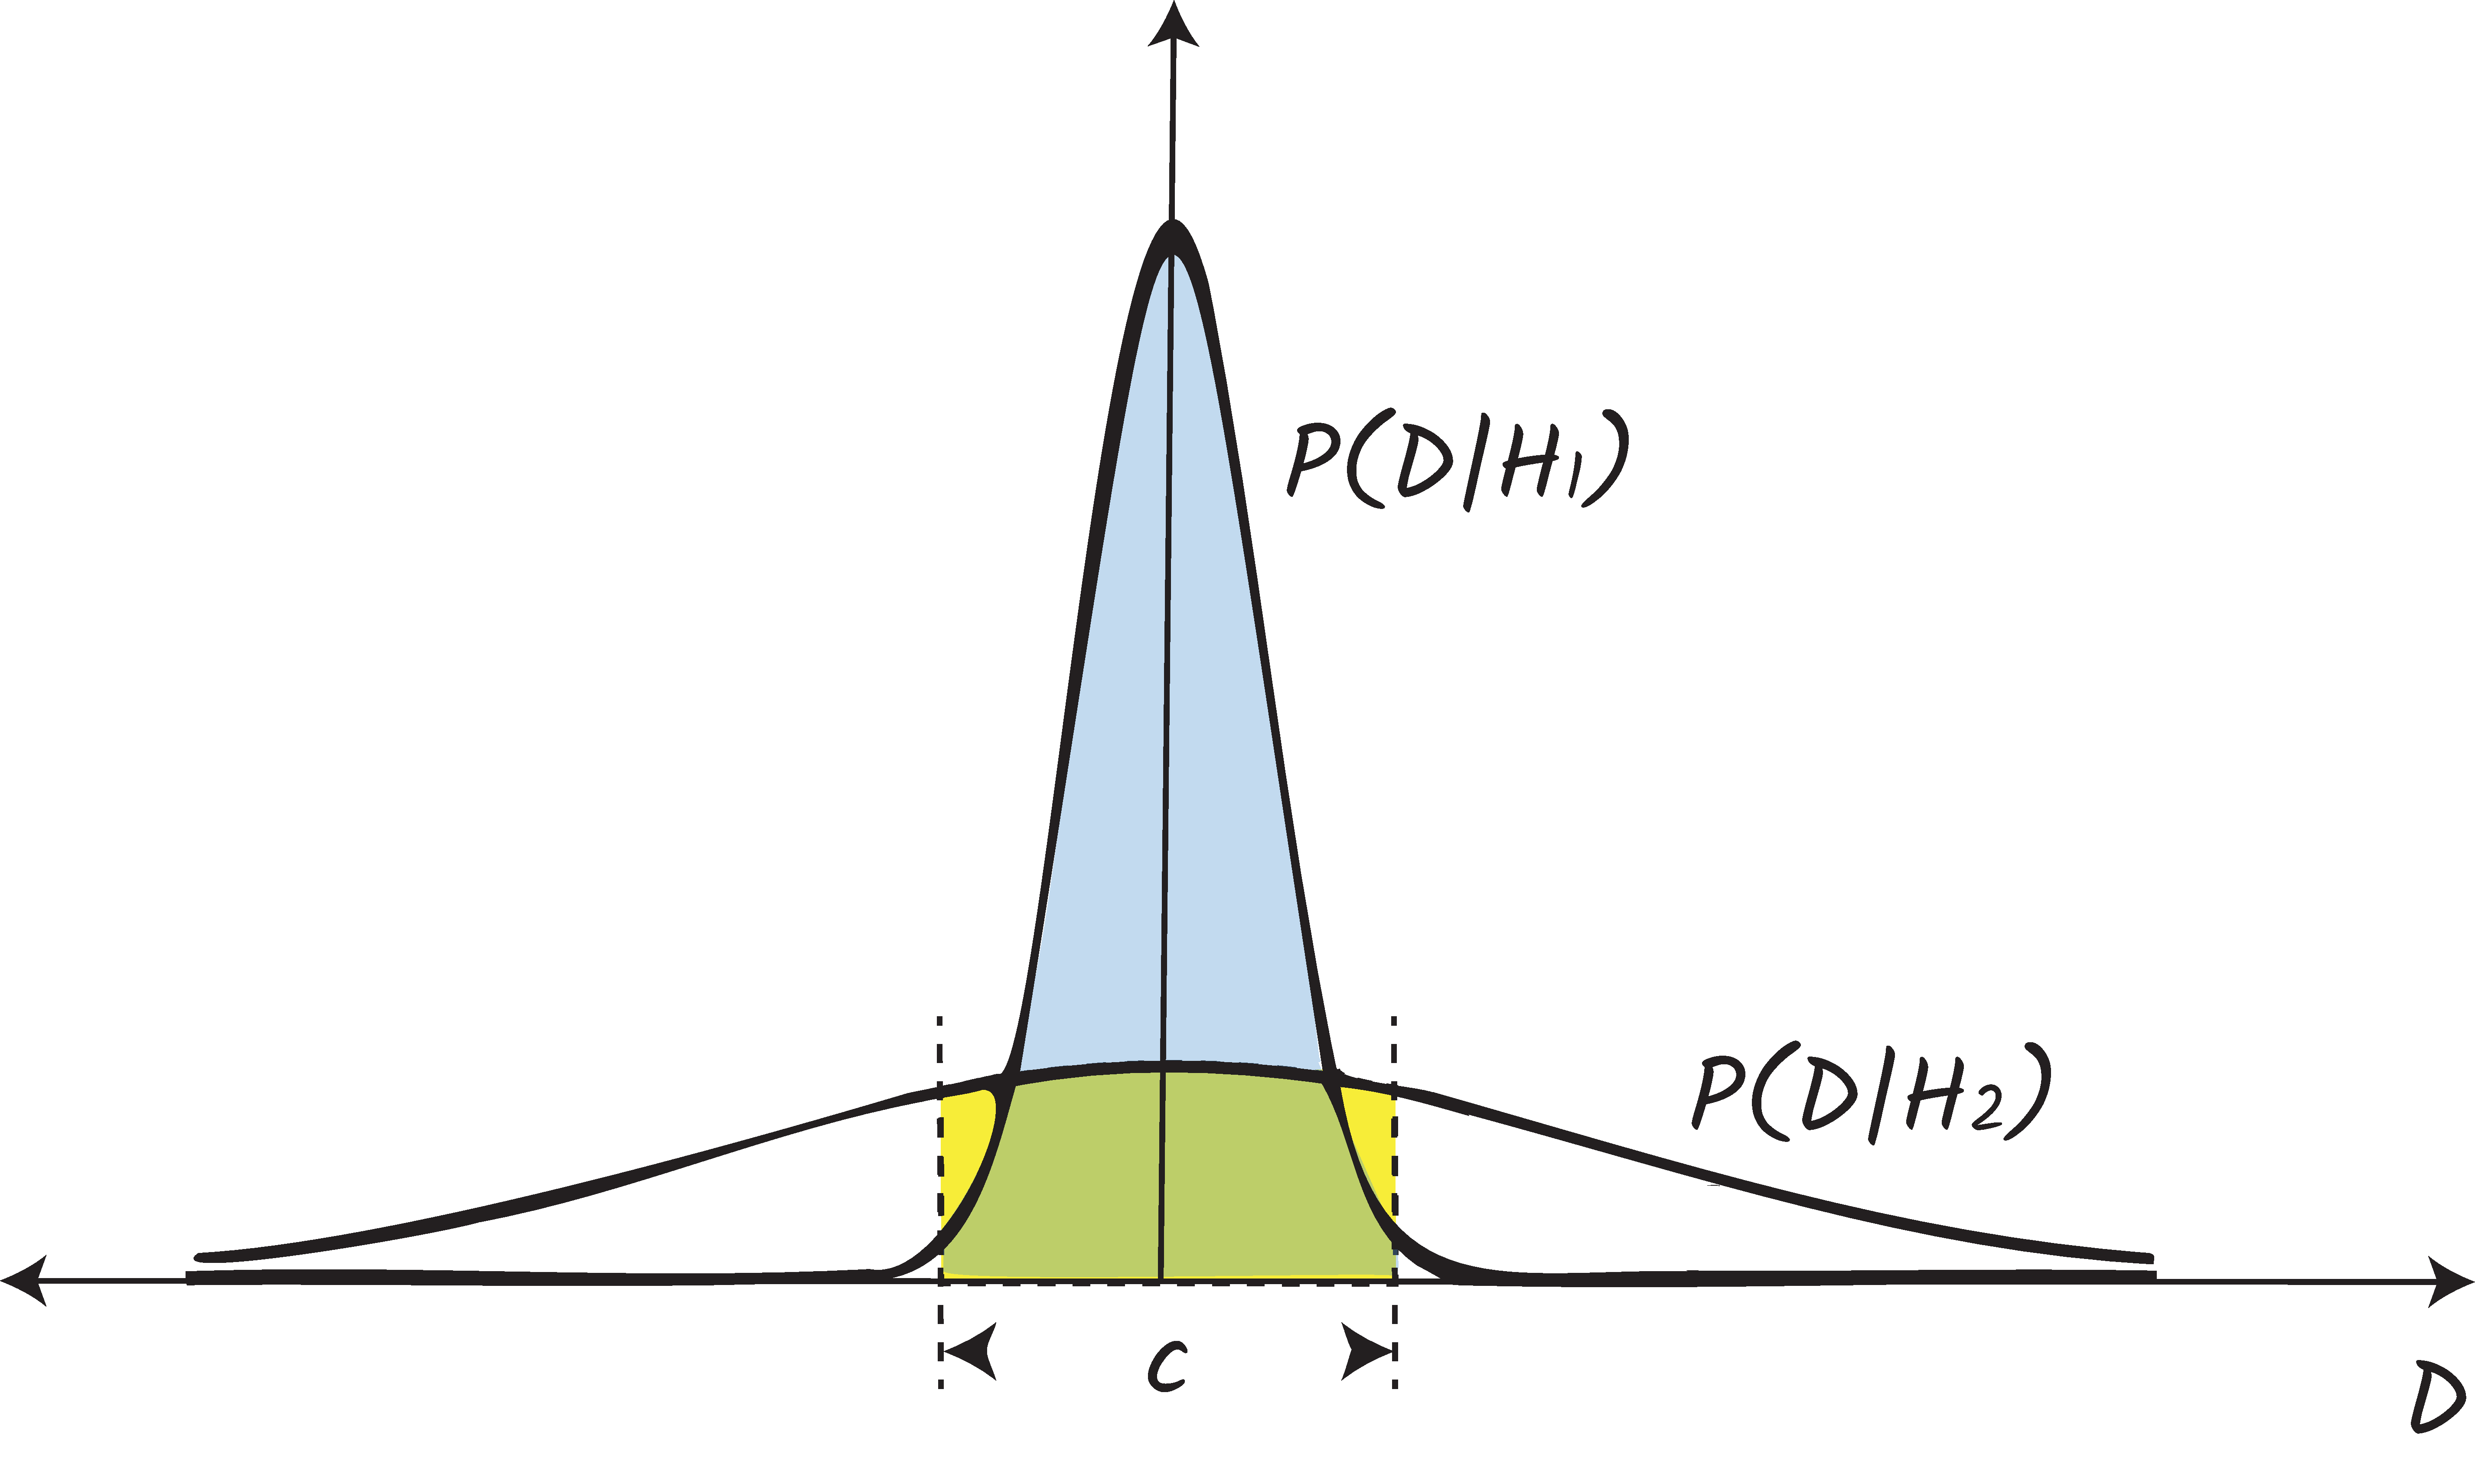
\includegraphics[width=0.75\linewidth]{model_comparison}
	\caption{Comparing models $\HH_1$ and $\HH_2$.}\label{modelcomparison}
	\end{figure}
	\begin{align}
    \frac{P(\HH_1|\DD)}{P(\HH_2|\DD)}&=\frac{P(\HH_1)}{P(\HH_2)}\frac{P(\DD|\HH_1)}{P(\DD|\HH_2)}\\
    \therefore P(\HH_1)&=P(\HH_1),~\text{no model bias} \to  \nonumber\\
		\frac{P(\HH_1|\DD)}{P(\HH_2|\DD)}&=\frac{P(\DD|\HH_1)}{P(\DD|\HH_2)}\label{evidence_comparisson}
   \end{align}

	Simple models make precise predictions, while complex models are capable of making a greater variety of predictions (\cref{modelcomparison}).

	If $\HH_2$ is more complex, it spread its predictive probability over a larger region of the data space $\DD$ than $\HH_1$. When both are compatible with the data, the simpler will turn out more probable than the complexer, despite any model preference.
 \subsection{Quantifying the Occam's razor}
 We already established that we can rank models based by evaluating the evidence$P(\DD|\HH_i)$  (\eqref{evidence_comparisson}) :
 \begin{align}
	P(\DD|\HH_i) = \int P(\DD|\vw, \HH_i) P(\vw|\HH_i) d\vw \label{evidence_integral}
\end{align}
Taking for simplicity the one-dimensional case and applying Laplace's method, we can approximate the evidance by multiplying the peak of $P(\DD|\HH_i)$ by $\sigma_{\vw|\DD}$:
\begin{align}
	\underbrace{P(\DD|\HH_i)}_\text{Evidence} \simeq \underbrace{P(\DD|\vw_{\text{\tiny MP}}, \HH_i)}_\text{Best-fit likelihood} \times \underbrace{P(\vw_{\text{\tiny MP}}|\HH_i) \sigma_{\vw|\DD}}_\text{Occam's factor}
\end{align}
The Occam's factor is the amount by which the accesible volume of $\HH_i$'s hypothesis space collapses when data arrive. This relates to how we measure information (\cref{guessing_game}).
The log of the Occam's factor is a measure of the amount of information we gain about the model's parameteres when data arrive~\cite{mackay:2002}.

The Occam's factor is the basis of \citeauthor{mackay:2002}'s Evidence Framework. The connection was no surprise given that we derived Information from the Bayesian interpretation of Probability (\cref{sec:prob2info}).
\section{Concluding Remarks}
